\documentclass[12pt,a4paper,titlepage]{article}
\title{Sound Event Detection con la tecnica del ``few-shot learning''} 
\author{Matteo Orlandini e Jacopo Pagliuca}
\date{\today}

\usepackage[english, italian]{babel} %the last declared language is the one used in the document
\usepackage[utf8]{inputenc}
\usepackage[T1]{fontenc}
\usepackage{booktabs} %toprule, midrule, bottomrule
\usepackage{subfig}
\usepackage{graphicx}
\usepackage{listings}
\usepackage{siunitx}
\usepackage{amsmath,amssymb}
\usepackage{xcolor}

\colorlet{punct}{red!60!black}
\definecolor{background}{HTML}{EEEEEE}
\definecolor{delim}{RGB}{20,105,176}
\colorlet{numb}{magenta!60!black}

\lstdefinelanguage{json}{
	basicstyle=\scriptsize,
	%numbers=left,
	tabsize=2,
	numberstyle=\scriptsize,
	stepnumber=1,
	numbersep=8pt,
	breaklines=true,
	frame=single,
	backgroundcolor=\color{background},
	literate=
	%*{0}{{{\color{numb}0}}}{1}
	%{1}{{{\color{numb}1}}}{1}
	%{2}{{{\color{numb}2}}}{1}
	%{3}{{{\color{numb}3}}}{1}
	%{4}{{{\color{numb}4}}}{1}
	%{5}{{{\color{numb}5}}}{1}
	%{6}{{{\color{numb}6}}}{1}
	%{7}{{{\color{numb}7}}}{1}
	%{8}{{{\color{numb}8}}}{1}
	%{9}{{{\color{numb}9}}}{1}
	%{:}{{{\color{punct}{:}}}}{1}
	{,}{{{\color{punct}{,}}}}{1}
	{\{}{{{\color{delim}{\{}}}}{1}
	{\}}{{{\color{delim}{\}}}}}{1}
	{[}{{{\color{delim}{[}}}}{1}
	{]}{{{\color{delim}{]}}}}{1},
 	morekeywords = {folder, reader_name, word, frequency, start, end, words, folders},
	keywordstyle=\bfseries\color{blue},
	commentstyle=\color{black},
	keepspaces=false,
	showspaces=false,
	showstringspaces=false,
}

\usepackage{color}
\definecolor{gray}{rgb}{0.4,0.4,0.4}
\definecolor{darkblue}{rgb}{0.0,0.0,0.6}
\definecolor{cyan}{rgb}{0.0,0.6,0.6}

\lstset{literate=
		{á}{{\'a}}1 {é}{{\'e}}1 {í}{{\'i}}1 {ó}{{\'o}}1 {ú}{{\'u}}1
		{Á}{{\'A}}1 {É}{{\'E}}1 {Í}{{\'I}}1 {Ó}{{\'O}}1 {Ú}{{\'U}}1
		{à}{{\`a}}1 {è}{{\`e}}1 {ì}{{\`i}}1 {ò}{{\`o}}1 {ù}{{\`u}}1
		{À}{{\`A}}1 {È}{{\'E}}1 {Ì}{{\`I}}1 {Ò}{{\`O}}1 {Ù}{{\`U}}1
		{ä}{{\"a}}1 {ë}{{\"e}}1 {ï}{{\"i}}1 {ö}{{\"o}}1 {ü}{{\"u}}1
		{Ä}{{\"A}}1 {Ë}{{\"E}}1 {Ï}{{\"I}}1 {Ö}{{\"O}}1 {Ü}{{\"U}}1
		{â}{{\^a}}1 {ê}{{\^e}}1 {î}{{\^i}}1 {ô}{{\^o}}1 {û}{{\^u}}1
		{Â}{{\^A}}1 {Ê}{{\^E}}1 {Î}{{\^I}}1 {Ô}{{\^O}}1 {Û}{{\^U}}1
		{ã}{{\~a}}1 {ẽ}{{\~e}}1 {ĩ}{{\~i}}1 {õ}{{\~o}}1 {ũ}{{\~u}}1
		{Ã}{{\~A}}1 {Ẽ}{{\~E}}1 {Ĩ}{{\~I}}1 {Õ}{{\~O}}1 {Ũ}{{\~U}}1
		{œ}{{\oe}}1 {Œ}{{\OE}}1 {æ}{{\ae}}1 {Æ}{{\AE}}1 {ß}{{\ss}}1
		{ű}{{\H{u}}}1 {Ű}{{\H{U}}}1 {ő}{{\H{o}}}1 {Ő}{{\H{O}}}1
		{ç}{{\c c}}1 {Ç}{{\c C}}1 {ø}{{\o}}1 {å}{{\r a}}1 {Å}{{\r A}}1
		{€}{{\euro}}1 {£}{{\pounds}}1 {«}{{\guillemotleft}}1
		{»}{{\guillemotright}}1 {ñ}{{\~n}}1 {Ñ}{{\~N}}1 {¿}{{?`}}1 {¡}{{!`}}1 
}

\lstdefinelanguage{XML}
{
	basicstyle=\tiny,	
	tabsize=2,
	frame=single,
	morestring=[b]",
	%morestring=[s]{>}{<},
	%morecomment=[s]{<?}{?>},
	stringstyle=\color{darkblue},
	identifierstyle=\color{cyan},
	keywordstyle=\bfseries\color{black},
	morekeywords={key, value, group, text, pronunciation, start, end}
	moreidentifier = {article, meta, link, prop, d, extra, t, s, n, ignored},
	backgroundcolor=\color{background},
	emph={key,end},          % Custom highlighting
	emphstyle=\bfseries\color{black},    % Custom highlighting style
	keepspaces=false,
	showspaces=false,
	showstringspaces=false,
	breaklines=true,         
	breakatwhitespace=false,  
}

\definecolor{maroon}{cmyk}{0, 0.87, 0.68, 0.32}
\definecolor{halfgray}{gray}{0.55}
\definecolor{ipython_frame}{RGB}{207, 207, 207}
\definecolor{ipython_bg}{RGB}{247, 247, 247}
\definecolor{ipython_red}{RGB}{186, 33, 33}
\definecolor{ipython_green}{RGB}{0, 128, 0}
\definecolor{ipython_cyan}{RGB}{64, 128, 128}
\definecolor{ipython_purple}{RGB}{170, 34, 255}


\lstdefinelanguage{iPython}{
	morekeywords={access,and,break,class,continue,def,del,elif,else,except,exec,finally,for,from,global,if,import,in,is,lambda,not,or,pass,print,raise,return,try,while},%
	%
	% Built-ins
	morekeywords=[2]{abs,all,any,basestring,bin,bool,bytearray,callable,chr,classmethod,cmp,compile,complex,delattr,dict,dir,divmod,enumerate,eval,execfile,file,filter,float,format,frozenset,getattr,globals,hasattr,hash,help,hex,id,input,int,isinstance,issubclass,iter,len,list,locals,long,map,memoryview,next,object,oct,open,ord,pow,property,range,raw_input,reduce,reload,repr,reversed,round,set,setattr,slice,sorted,staticmethod,str,sum,super,tuple,type,unichr,unicode,vars,xrange,zip,apply,buffer,coerce,intern, F, nn, np},%
	%
	sensitive=true,%
	morecomment=[l]\#,%
	morestring=[b]',%
	morestring=[b]",%
	%
	morestring=[s]{'''}{'''},% used for documentation text (mulitiline strings)
	morestring=[s]{"""}{"""},% added by Philipp Matthias Hahn
	%
	morestring=[s]{r'}{'},% `raw' strings
	morestring=[s]{r"}{"},%
	morestring=[s]{r'''}{'''},%
	morestring=[s]{r"""}{"""},%
	morestring=[s]{u'}{'},% unicode strings
	morestring=[s]{u"}{"},%
	morestring=[s]{u'''}{'''},%
	morestring=[s]{u"""}{"""},%
	%
	% {replace}{replacement}{lenght of replace}
	% *{-}{-}{1} will not replace in comments and so on
	literate=
	{á}{{\'a}}1 {é}{{\'e}}1 {í}{{\'i}}1 {ó}{{\'o}}1 {ú}{{\'u}}1
	{Á}{{\'A}}1 {É}{{\'E}}1 {Í}{{\'I}}1 {Ó}{{\'O}}1 {Ú}{{\'U}}1
	{à}{{\`a}}1 {è}{{\`e}}1 {ì}{{\`i}}1 {ò}{{\`o}}1 {ù}{{\`u}}1
	{À}{{\`A}}1 {È}{{\'E}}1 {Ì}{{\`I}}1 {Ò}{{\`O}}1 {Ù}{{\`U}}1
	{ä}{{\"a}}1 {ë}{{\"e}}1 {ï}{{\"i}}1 {ö}{{\"o}}1 {ü}{{\"u}}1
	{Ä}{{\"A}}1 {Ë}{{\"E}}1 {Ï}{{\"I}}1 {Ö}{{\"O}}1 {Ü}{{\"U}}1
	{â}{{\^a}}1 {ê}{{\^e}}1 {î}{{\^i}}1 {ô}{{\^o}}1 {û}{{\^u}}1
	{Â}{{\^A}}1 {Ê}{{\^E}}1 {Î}{{\^I}}1 {Ô}{{\^O}}1 {Û}{{\^U}}1
	{œ}{{\oe}}1 {Œ}{{\OE}}1 {æ}{{\ae}}1 {Æ}{{\AE}}1 {ß}{{\ss}}1
	{ç}{{\c c}}1 {Ç}{{\c C}}1 {ø}{{\o}}1 {å}{{\r a}}1 {Å}{{\r A}}1
	{€}{{\EUR}}1 {£}{{\pounds}}1
	%
	{^}{{{\color{ipython_purple}\^{}}}}1
	{=}{{{\color{ipython_purple}=}}}1
	%
	{+}{{{\color{ipython_purple}+}}}1
	{*}{{{\color{ipython_purple}$^\ast$}}}1
	{/}{{{\color{ipython_purple}/}}}1
	%
	{+=}{{{+=}}}1
	{-=}{{{-=}}}1
	{*=}{{{$^\ast$=}}}1
	{/=}{{{/=}}}1,
	literate=
	*{-}{{{\color{ipython_purple}-}}}1
	{?}{{{\color{ipython_purple}?}}}1,
	%
	identifierstyle=\color{black}\ttfamily,
	commentstyle=\color{ipython_cyan}\ttfamily,
	stringstyle=\color{ipython_red}\ttfamily,
	keepspaces=false,
	showspaces=false,
	breaklines=true,
	showstringspaces=false,
	%
	rulecolor=\color{ipython_frame},
	frame=single,
	frameround={t}{t}{t}{t},
	framexleftmargin=6mm,
	numbers=left,
	numberstyle=\tiny\color{halfgray},
	%
	%
	backgroundcolor=\color{ipython_bg},
	%   extendedchars=true,
	basicstyle=\scriptsize,
	tabsize=1,
	keywordstyle=\color{ipython_green}\ttfamily,
	morekeywords={typeof, null, catch, switch, in, int, str, float, self, import, def, return, True, False, None},
	emph={read_json_file,write_json_file, exists, parse, getroot, basename, scandir, keys, Counter, append, sample, isdir, compute_melspectrogram, load, melspectrogram,power_to_db, mkdir, save_dataset, save_test_dataset, OSError, find_valid_readers, create_training_validation_test_readers, find_classes, concatenate, FloatTensor, save, load, tqdm, empty, count_parameters, conv_block, Protonet, Module, init,Sequential, forward, is_available, Adam, get_training_validation_readers, trange, batch_sample, to, train, zero_grad, loss, backward, step, batch_sample, mean, savemat,get_training_validation_readers, empty, shape, cat, unsqueeze, expand, squeeze, size, arange, view, expand, mean, euclidean_dist, log_softmax, gather, eq, max, min, Adam, load_state_dict, isfile, listdir, get_negative_positive_query_set, test_predictions, cpu, tolist, precision_recall_curve, auc, std, get_negative_positive_query_set, test_predictions, size, softmax, detach, reshape, squeeze, Sequential, Conv2d, BatchNorm2d, ReLU, MaxPool2d, Linear, normal_,sigmoid,relu,zero_,fill_,sqrt,get_device_properties, interpolate, repeat, unsqueeze, transpose, },          % Custom highlighting
	emphstyle=\color{ipython_purple}\ttfamily,    % Custom highlighting style
}

%\usepackage[latin1]{inputenc} %l'ho messo io (Jacopo)
%inizio impostazioni bibliografia
\usepackage[autostyle,italian=guillemets]{csquotes} 
%autostyle adatta lo stile delle citazioni alla lingua corrente del documento;
%italian=guillemets racchiude automaticamente tra virgolette caporali
%i campi che prevedono le virgolette;
\usepackage[backend=biber, style=numeric, citestyle=numeric,maxcitenames=99,maxbibnames = 99]{biblatex}
%backend=biber dice a biblatex che s’intende usare Biber come motore bibliografico
%style:numeric Anno di pubblicazione: in fondo al riferimento.
%citestyle=numeric Riferimento: numerico ([1], [2], eccetera).
%fine impostazioni bibliografia

\usepackage{float}
\usepackage{hyperref}
\hypersetup{
%	bookmarks=true,         % show bookmarks bar?
	unicode=false,          % non-Latin characters in Acrobat’s bookmarks
	pdftoolbar=true,        % show Acrobat’s toolbar?
	pdfmenubar=true,        % show Acrobat’s menu?
	pdffitwindow=false,     % window fit to page when opened
	pdfstartview={FitH},    % fits the width of the page to the window
	%pdftitle={Relazione di Reti di Sensori Wireless per IOT},    % title
	pdfauthor={Matteo Orlandini},     % author
	pdfsubject= {Sound Event Detection con la tecnica del few-shot learning},   % subject of the document
	pdfcreator={Matteo Orlandini},   % creator of the document
	%pdfproducer={Producer}, % producer of the document
	pdfpagemode={UseOutlines},
	%bookmarksopen,
	pdfstartview={FitH},
	colorlinks=false,       % false: boxed links; true: colored links
	linkcolor={red},
	citecolor={green},
	urlcolor={cyan}
} 

\renewcommand{\lstlistingname}{Codice}

\addbibresource{Bibliografia.bib}

\newcommand{\CoverName}{Cover}

\begin{document}

\begin{titlepage}
	
	\centering
	
\includegraphics[width=.2\textwidth]{Immagini/univpmlogo}\par\vspace{1cm}
	{\scshape\LARGE Università Politecnica delle Marche\par}
	\vspace{1cm}
	{\scshape\Large Digital Adaptive Circuits And Learning Systems\par}
	\vspace{1.5cm}
	{\huge\bfseries Sound Event Detection con la tecnica del  ``\emph{few-shot learning}''  \par}
	\vspace{2cm}
	{\Large\itshape Matteo Orlandini e Jacopo Pagliuca\par}
	\vfill
	Prof. Stefano \textsc{Squartini}\\
	Dott.ssa Michela \textsc{Cantarini}
	
	\vfill
	
	% Bottom of the page
	{\large \today\par}
\end{titlepage}

\thispagestyle{empty}
\tableofcontents
\clearpage

%\newpage
\setcounter{page}{1}

\section{Introduzione}
\label{section:Introduzione}
Lo scopo della tesina è quello di riprodurre i risultati ottenuti nel paper ``\textit{Few-Shot Event Detection}''~\cite{Salamon:Few-Shot}.
L'argomento centrale dello studio è l'individuazione di eventi sonori percettivamente simili all'interno di una registrazione.
Varie applicazioni di questo algoritmo possono essere la rilevazione di particolari suoni nella musica o la rimozione di parole di riempimento nei podcast.
Solitamente questo processo avviene manualmente risultando in un compito difficile e tedioso.

I classici modelli di deep-learning per la determinazione di suoni richiedono una grande mole di dati per fare il training. In questo modo la rete è capace di riconoscere parole sulle quali si è allenata.

Nell'approccio few-shot invece, è necessario un piccolo dataset di riferimento. La rete non sarà allenata a riconoscere i suoni che ha ascoltato nel training, ma assumerà la capacità di riconoscere la somiglianza fra due suoni che sta analizzando.

Le reti few-shot di solito sono state utilizzate per un set chiuso dove in un \textit{task} di classificazione veniva presentata una query e confrontata con K istanze di C classi, con C fisso.
Questo metodo è chiamato C-way K-shot.

Il paper di riferimento invece, cerca di applicare una rete few-shot in un contesto più ampio in cui è necessario riconoscere una parola non vista in precedenza in una sequenza di suoni non classificati precedentemente dalla rete.

Per fare questo, l'idea è quella di costruire un set positivo e un set negativo con i quali confrontare la query, come mostrato in~\ref{fig:few_shot_sound_event_detection_method}. Mentre il set positivo è costituito da istanze della stessa parola, quello negativo comprende vari campioni di parole diverse e rappresenta un generico esempio di tutto ciò che non comprende la parola da cercare.

Prima di fare questo però, la rete deve ``\textit{imparare ad imparare}'': verrà quindi sottoposta a una serie di task classici di few shot nei quali la rete deve riconoscere a quale classe appartiene una query avendo come riferimento K istanze di C classi, che costituiscono il support set.

Il support set e la query può essere diverso ad ogni episodio, generalizzando il più possibile l'evento e allenando la capacità della rete di \textit{riconoscere la somiglianza} tra le parole, ma non le parole stesse.


\begin{figure}[h]
	\centering	
	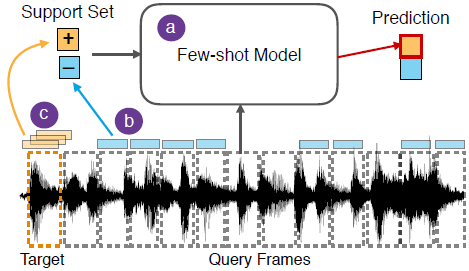
\includegraphics[width=.5\textwidth]{Immagini/few_shot_sound_event_detection_method}
	\caption{Metodo proposto per il few-shot sound event detection. (a) Applicazione del modello few-shot, (b) costruzione del set di esempi negativi, in blu, e (c) data augmentation per la generazioni di più esempi positivi, in arancione.~\cite{Salamon:Few-Shot}}
	\label{fig:few_shot_sound_event_detection_method}
\end{figure}

\begin{figure}[h]
	\centering	
	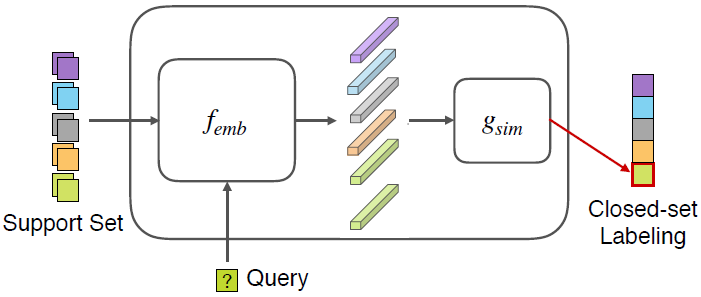
\includegraphics[width=.5\textwidth]{Immagini/few_shot_learning_model}
	\caption{Modello few-shot learning nel caso 5\emph{-way} 2\emph{-shot}.~\cite{Salamon:Few-Shot}}
	\label{fig:few-shot_learning_model}
\end{figure}
\clearpage

\section{Convolutional Neural Network (CNN)}
Una rete neurale convoluzionale è una rete feedforward pensata per applicazioni che richiedono l'elaborazione di immagini o di grandi moli di dati.
L'ingresso della rete è costituito da una o più matrici che attraversano dei blocchi convoluzionali che ne riducono le dimensioni. I filtri di convoluzione sono detti kernel. Infine, il risultato viene passato a una rete fully connected che ha il compito di classificazione.

La prima parte del filtro consiste nella convoluzione dell'immagine in ingresso con una serie di kernel i cui parametri vengono allenati.
Il filtro viene traslato in entrambe le dimensioni della matrice producendo una serie di feature bidimensionali.
Il parametro \textit{stride} definisce il passo con cui il kernel viene traslato sulla matrice di ingresso.
Solitamente, viene effettuato uno zero-padding sui contorni del volume in modo da poter caratterizzare anche i valori che si trovano ai bordi delle matrici.
In seguito alla convoluzione viene applicata una funzione non-lineare come ad esempio una sigmoide o una ReLu con lo scopo di aumentare la proprietà di non linearità.

Il pooling layer è uno strato della rete che ha lo scopo di ridurre le dimensioni della matrice prodotta dal convolutional layer. Combinando gruppi di elementi della matrice (solitamente $2 \times 2$) restituisce il valore massimo tra essi, che andrà a sostituire il blocco stesso.

\section{Few-shot learning}
\label{section:Few-shot}
\subsection{Introduzione}
Gli esseri umani possono riconoscere nuove classi di oggetti partendo da pochissimi esempi. Tuttavia, la maggior parte delle tecniche di machine learning richiedono migliaia di esempi per ottenere prestazioni simili a quelle umane. L'obiettivo del \textit{few-shot learning} è classificare i nuovi dati dopo aver visto solo pochi esempi di training. Nel caso estremo, potrebbe esserci solo un singolo esempio per ogni classe (\textit{one shot learning}). In pratica, il few-shot learning è utile quando è difficile trovare esempi di training (ad es. casi di una malattia rara) o quando l'etichettatura dei dati è onerosa.

L'apprendimento few-shot viene solitamente studiato utilizzando la classificazione \emph{C-way K-shot}. L'obiettivo è quello di discriminare le $C$ classi composte da $K$ esempi ciascuna. Una tipica dimensione del problema potrebbe essere quella di discriminare tra $C=10$ classi con solo $K=5$ campioni ciascuno di training. Non possiamo allenare un classificatore usando metodi convenzionali; qualsiasi algoritmo di classificazione moderno dipenderà da molti più parametri rispetto agli esempi di addestramento e generalizzerà male.

Se i dati non sono sufficienti per ridurre il problema, una possibile soluzione è acquisire esperienza da altri problemi simili. A tal fine, la maggior parte degli approcci caratterizza l'apprendimento a breve termine con un problema di meta-apprendimento.

\subsection{Struttura del meta learning}
Nell'apprendimento classico, impariamo come classificare dai dati di training e valutiamo i risultati utilizzando i dati di test. Nel quadro del meta-apprendimento, \textit{impariamo come imparare} a classificare in base a una serie di \textit{episodi di training} e valutiamo utilizzando una serie di episodi di test; In altre parole, usiamo un insieme di problemi di classificazione per aiutare a risolvere altri insiemi non correlati.

Qui, ogni attività imita lo scenario few-shot, quindi per la classificazione C-way-K-shot, ogni attività include C classi con K esempi ciascuna. Questi sono noti come support set e vengono utilizzati per apprendere come risolvere il task. Inoltre, esistono ulteriori esempi delle stesse classi, note come set di query, utilizzate per valutare le prestazioni dell'episodio corrente. Ogni episodio può essere completamente unico; potremmo non vedere mai le classi di un episodio in nessuno degli altri. L'idea è che il sistema veda ripetutamente istanze durante l'addestramento che corrispondono alla struttura dell'attività finale di few-shot, ma che contengono classi diverse.

Ad ogni fase del meta-apprendimento, aggiorniamo i parametri del modello in base ad un episodio di training selezionato casualmente. La funzione di loss è determinata dalle prestazioni di classificazione sul set di query dell'episodio, in base alla conoscenza acquisita dal relativo support set. Poiché la rete viene sottoposta ad un compito diverso in ogni fase temporale, deve imparare a discriminare le classi di dati in generale, piuttosto che un particolare sottoinsieme di classi.

Per valutare le prestazioni nel few-shot, utilizziamo una serie di attività di test. Ciascuna contiene solo classi invisibili che non erano in nessuna delle attività di formazione. Per ciascuno, misuriamo le prestazioni sul query set in base alla conoscenza del loro support set.


%\subsection{Approcci al meta-apprendimento}
%Gli approcci al meta-apprendimento sono diversi e non c'è consenso sull'approccio migliore. Tuttavia, esistono tre famiglie distinte, ognuna delle quali sfrutta un diverso tipo di conoscenza a priori:
%\begin{itemize}
%	\item Conoscenze a priori sulla somiglianza: apprendiamo degli embedding nei training task che tendono a separare classi diverse anche quando non sono visibili.
%	\item Conoscenze a priori sull'apprendimento: utilizziamo le conoscenze a priori per vincolare l'algoritmo di apprendimento a scegliere parametri che generalizzino bene da pochi esempi.
%	\item Conoscenza a priori dei dati: sfruttiamo le conoscenze a priori sulla struttura e la variabilità dei dati e questo ci consente di apprendere modelli praticabili da pochi esempi.
%\end{itemize}

\section{Prototypical Network}
L'approccio si basa sull'idea che esista un embedding in cui i punti delle istanze di una classe si raggruppano attorno a una singola rappresentazione per ogni classe, chiamata \textit{prototipo}. 
Nella classificazione few-shot per ogni episodio viene fornito un support set di $N$ esempi etichettati  $S=\{(\mathbf{x}_1,y_1), \dots,(\mathbf{x}_N,y_N)\}$ dove $\mathbf{x}_i\in \mathbb{R}^D$ rappresenta il vettore $D$-dimensionale della feature (nel nostro caso spettrogrammi di dimensione $128 \times 51$) e $y_i \in \{1, \dots, K\}$ la rispettiva label. $S_k$ denota il set di esempi etichettati con la classe $k$.

La rete Prototypical calcola una rappresentazione $M$-dimensionale $\mathbf{c}_k$, o \emph{prototipo}, di ogni classe tramite una funzione di embedding $f_\phi : \mathbb{R}^D \rightarrow \mathbb{R}^M$ con parametri da allenare $\phi$. La funzione di embedding è rappresentata da una rete convoluzionale. Ogni prototipo è calcolato come la media tra gli embedding delle istanze della stessa classe.
\begin{equation}
	\mathbf{c}_k=\frac{1}{|S_k|}\sum_{(\mathbf{x}_i,y_i)\in S_k}f_\phi (\mathbf{x}_i)
\end{equation}
Data una funzione distanza $d: \mathbb{R}^M \times \mathbb{R}^M \rightarrow [0, +\infty )$, la rete Protypical calcola la relazione di una query $\mathbf{x}$ rispetto ai prototipi tramite la funzione softmax delle distanze prese con segno negativo.
\begin{equation}\label{eq:softmax}
p_\phi(y=k|\mathbf{x})=\dfrac{\exp(-d(f_\phi(\mathbf{x}),\mathbf{c}_k))}{\sum_k' \exp(-d(f_\phi(\mathbf{x}),\mathbf{c}_k'))}
\end{equation}
Il processo di training avviene minimizzando il negativo del logaritmo della probabilità
\begin{equation}\label{eq:loss_proto}
	J(\phi)=-\log\left(p_\phi(y=k|\mathbf{x})\right)
\end{equation}
considerando la distanza fra query e il prototipo della sua classe.
Gli episodi di training sono formati campionando C classi di parole da un lettore e selezionando per ognuna casualmente K istanze e Q query.

\begin{figure}[h]
	\centering
	{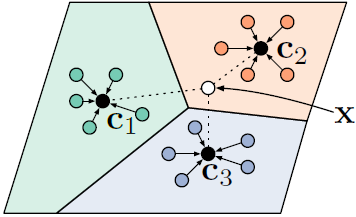
\includegraphics[width=0.5\textwidth]{Immagini/proto_few_shot}}
	\label{fig:proto_few_zero_shot}	
	\caption{I prototipi few-shot $\mathbf{c}_k$ sono calcolati come la media degli embedding del support set per ogni classe. I punti degli embedding delle query sono classificati facendo il softmax sulle distanze del prototipo delle classi: $p_\phi(y = k|\mathbf{x}) \propto \exp \left(-d(f_\phi(\mathbf{x}),\mathbf{c}_k) \right)$.~\cite{snell:prototypical}}
\end{figure}
\clearpage

\section{Relation Network}
La rete Relation ha lo scopo di associare due istanze alla volta per determinare la loro similarità.
Questo viene effettuato concatenando gli embedding di più istanze in un unico elemento che sarà dato in ingresso a una rete decisionale i cui parametri saranno aggiornati in modo che una concatenazione di elementi simili restituisca un risultato vicino a 1.
La Relation Network è costituita da due moduli: un modulo di \emph{embedding} $f_\varphi$ (equivalente a quello nella Prototypical) e un modulo di \emph{relation} $g_\phi$, come illustrato in figura~\ref{fig:relation_network}.
Le istanze $x_i$ del query set $\mathcal{Q}$ e quelle $x_j$ del support set $\mathcal{S}$ vengono date in ingresso al modulo di embedding producendo dei vettori (feature maps) $f_\varphi(x_i)$ e $f_\varphi(x_j)$.
Questi ultimi vengono poi dati all'operatore $\mathcal{C}(\cdot ,\cdot)$ che ne fa la concatenazione: $\mathcal{C}(f_\varphi(x_i),f_\varphi(x_j))$.
Le feature map concatenate passano poi attraverso il modulo di decisione che restituisce uno scalare da 0 a 1, il quale rappresenta la somiglianza tra $x_i$ e $x_j$.
Per il caso $C$-way one-shot, viene concatenata la query con le istanze delle $C$ classi producendo $C$ punteggi di somiglianza.
\begin{equation}
	r_{i,j}=g_\phi(\mathcal{C}(f_\varphi(x_i),f_\varphi(x_j))),  \qquad i = 1, 2, \dots, C
\end{equation}
Nel caso $C$-way K-shot invece, la query viene concatenata con la somma elemento per elemento degli embedding di ogni istanza delle classi. Quindi, in entrambi i casi i confronti $r_{i,j}$ sono $C$ per ogni query.

Per allenare il modello viene usato l'errore quadratico medio (MSE) in modo che l'uscita del modulo di decisione produca 1 se i vettori concatenati sono della stessa classe e 0 altrimenti.

\begin{figure}[h]
	\centering	
	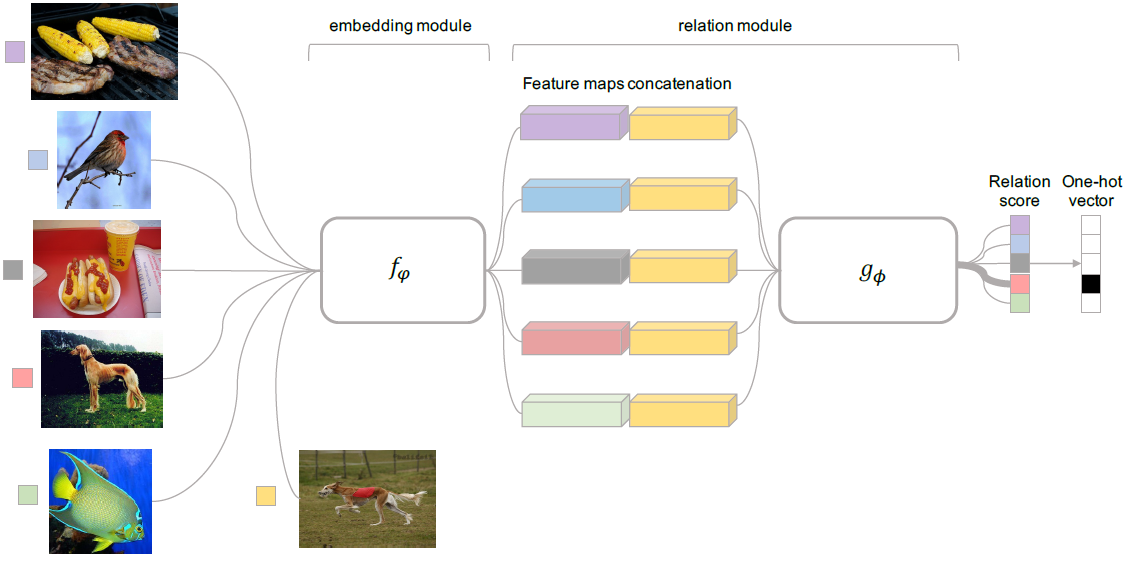
\includegraphics[width=0.8\textwidth]{Immagini/relation_network}
	\caption{Architettura della Relation Network nel caso 5\emph{-way} 1\emph{-shot} con un esempio di query.~\cite{DBLP:journals/corr/abs-1711-06025}}
	\label{fig:relation_network}
\end{figure}

\begin{figure}[h]
	\centering
	\subfloat[Blocco convoluzionale\label{fig:relation_network_architecture_a}]{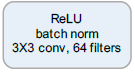
\includegraphics[width=0.3\textwidth]{Immagini/relation_network_conv_block}}
	\qquad
	\subfloat[Relation Network per few-shot learning\label{fig:relation_network_architecture_b}]{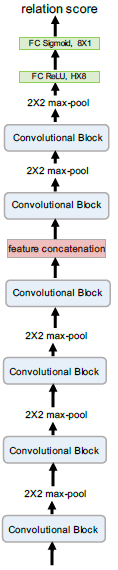
\includegraphics[width=0.25\textwidth]{Immagini/relation_network_architecture}}
	\label{fig:relation_network_architecture}	
	\caption{Architettura della Relation Network per few-shot learning (b) composta dagli elementi inclusi nel blocco convoluzionale (a).~\cite{DBLP:journals/corr/abs-1711-06025}}
\end{figure}

\clearpage

\section{Preprocessing del dataset}
\label{sec:preprocessing_dataset}
\subsection{Dataset Spoken Wikipedia Corpora}
\label{subsec:spoken_wikipedia_corpora}
Il progetto Spoken Wikipedia unisce lettori volontari di articoli di Wikipedia. Sono disponibili centinaia di articoli in inglese, tedesco e olandese per gli utenti che non sono in grado o non vogliono leggere la versione scritta dell'articolo. Il dataset trasforma i file audio in un corpus, cioè una raccolta ordinata e completa di opere o di autori, allineato nel tempo, rendendolo accessibile per la ricerca.\cite{minining_spoken_wikipedia}

Questo corpus ha diverse caratteristiche importanti:
\begin{itemize}
	\item centinaia di ore di audio allineato
	\item lettori eterogenei
	\item diversi argomenti
	\item genere testuale ben studiato
	\item le annotazioni delle parole possono essere mappate all'html originale
	\item allineamenti a livello di fonema
\end{itemize}

Ogni articolo è suddiviso in sezioni, frasi e token. Ogni token è normalizzato e la normalizzazione è allineata all'audio.

\subsection{Le annotazioni del dataset}
\label{subsec:annotazioni}
Ogni annotazione è racchiusa in un tag chiamato ``\texttt{article}'', che contiene una sezione ``\texttt{meta}'' per i metadati, come si può vedere in~\ref{metadati_annotazioni} e una sezione ``\texttt{d}'', come in~\ref{annotazioni}, contenente l'articolo e le relative annotazioni.

\begin{lstlisting}[language=XML,firstnumber=1, caption=Metadati delle annotazioni delle parole in un audio, label=metadati_annotazioni,captionpos=b]
<article>
	<meta>
		<link key="DC.conformsto" value="http://nats.gitlab.io/swc/schema/swc-1.0.rnc"/>
		<prop key="DC.creator" value="Spoken Wikipedia Corpus Collection Software"/>
		<prop key="DC.publisher" value="Universität Hamburg"/>
		<link key="DC.reference" value="http://nbn-resolving.de/urn:nbn:de:gbv:18-228-7-2209"/>
		<prop key="DC.type" value="dataset"/>
		<prop key="DC.license" value="CC-BY-SA"/>
		<prop key="DC.title" value="Limerence"/>
		<prop key="DC.language" value="en"/>
		<prop key="DC.identifier" value="Limerence"/>
		<prop key="DC.date.read" value="2005-04-29 00:00:00"/>
		<link key="DC.source" value="https://en.wikipedia.org/wiki/Limerence"/>
		<prop key="DC.source.wikiID" value="154147"/>
		<prop key="DC.source.revision" value="791627969"/>
		<link key="DC.source.text" value="https://en.wikipedia.org/w/index.php?title=Limerence&oldid=13811989"/>
		<link key="DC.source.audio" value="https://upload.wikimedia.org/wikipedia/commons/a/aa/Limerence.ogg" group="audio1"/>
		<prop key="DC.source.audio.offset" value="0.0" group="audio1"/>
		<link key="DC.source.audio.page" value="https://en.wikipedia.org/w/index.php?title=File%3aLimerence.ogg" group="audio1"/>
		<link key="DC.source.audio.date" value="2007-09-14 19:23:05" group="audio1"/>
		<prop key="reader.name" value="the Epopt"/>
		<prop key="processing.step" value="tokenize" group="tokenize"/>
		<prop key="processing.step.date" value="2017-08-10T07:44:44.095+02:00[Europe/Berlin]" group="tokenize"/>
		<prop key="processing.step.options" value="Namespace(output=articles/Limerence/tokenized.swc, all_sections=false, null_normalize=false, raw_output=null, subparser_name=tokenize, lang=en, no_introduction=false, article_dir=articles/Limerence)" group="tokenize"/>
		<prop key="processing.step.git.commit.id" value="7431dbf93f212ad828208abaf8f518fb8de11ff3" group="tokenize"/>
		<prop key="processing.step.git.commit.time" value="09.08.2017 @ 15:21:55 CEST" group="tokenize"/>
		<prop key="processing.step" value="align" group="align"/>
		<prop key="processing.step.date" value="2017-08-11T16:12:18.423+02:00[Europe/Berlin]" group="align"/>
		<prop key="processing.step.options" value="Namespace(output=articles/Limerence/aligned.swc, transcript=articles/Limerence/tokenized.swc, g2p=../model_en/model.fst.ser, phone=false, subparser_name=align, dict=../model_en/empty.dic, acoustic_model=../model_en/, audio=articles/Limerence/audio.wav)" group="align"/>
		<prop key="processing.step.git.commit.id" value="7431dbf93f212ad828208abaf8f518fb8de11ff3" group="align"/>
		<prop key="processing.step.git.commit.time" value="09.08.2017 @ 15:21:55 CEST" group="align"/>
	</meta>
\end{lstlisting}
Il documento, contrassegnato dal tag ``\texttt{d}'', può contenere parti diverse, ciascuna spiegata di seguito. La sezione ``\texttt{extra}'' contiene il testo che abbiamo incluso ma non fa parte dell'articolo, ``\texttt{ignored}'' contiene ciò che fa parte del testo ma viene ignorato per l'allineamento, ``\texttt{section}'' contiene un titolo e un contenuto, ``\texttt{p}'' contiene un paragrafo  e ``\texttt{s}'' una frase che a sua volta contiene dei token ``\texttt{t}''. In quest'ultimo è contenuta la singola parola originale e le normalizzazioni. Per esempio, la punteggiatura non ha annotazioni di normalizzazione in quanto non è pronunciata, ma il numero 500 ne ha due - ``cinque'' e ``cento''. un token stesso non ha allineamento, solo la sua normalizzazione ``\texttt{n}'' è allineata. La normalizzazione ha una ``\texttt{pronunciation}'' e può avere un tempo di ``\texttt{start}'' ed ``\texttt{end}'', se è allineata. La normalizzazione, a sua volta, può contenere dei fonemi ``\texttt{ph}''.

\begin{lstlisting}[language=XML,firstnumber=1, caption=Annotazioni delle parole in un audio, label=annotazioni,captionpos=b]
<d>
	<extra text="LimerenceFrom wikipedia, the free encyclopedia at e n dot wikipedia dot org.">
		<s text="LimerenceFrom wikipedia, the free encyclopedia at e n dot wikipedia dot org.">
			<t text="LimerenceFrom">
				<n pronunciation="LimerenceFrom" start="140" end="1190"/>
			</t>
			<t text="wikipedia">
				<n pronunciation="wikipedia" start="1250" end="1950"/>
			</t>
			<t text=","/>
			<t text="the">
				<n pronunciation="the" start="1950" end="2070"/>
			</t>
			<t text="free">
				<n pronunciation="free" start="2070" end="2300"/>
			</t>
			<t text="encyclopedia">
				<n pronunciation="encyclopedia" start="2300" end="3220"/>
			</t>
			<t text="at">
				<n pronunciation="at"/>
			</t>
			<t text="e">
				<n pronunciation="e" start="3490" end="3710"/>
			</t>
\end{lstlisting}

\subsection{Lettori del dataset}
\label{subsec:lettori}
Il dataset Spoken Wikipedia Corpora contiene un totale di 1340 audio di diversi lettori, ma nel progetto vengono presi solo gli audio che contengono annotazioni a livello di parola. In questo modo vengono presi solo 208 lettori e partizionati come in~\cite{Salamon:Few-Shot} con un rapporto $138:15:30$ tra lettori di training, validation e test. I lettori e le parole sono state estratte dai file ``aligned.swc'' contenuti in ogni audio e, successivamente, salvati in diversi file json. Per la gestione dei json sono state create due funzioni utili per la lettura e scrittura come mostrato nel codice~\ref{json_manager}.
\begin{lstlisting}[language=iPython,firstnumber=1, caption=json\_manager.py, label=json_manager,captionpos=b]
import json
	
def write_json_file(filename, list_of_dict, indent = 0):
	f = open(filename, "w")
	f.write(json.dumps(list_of_dict, indent = indent))
	f.close
	
def read_json_file(filename):
	f = open(filename, "r")
	list_of_dict = json.load(f)
	f.close
	return list_of_dict
\end{lstlisting}

Il codice~\ref{xml_parser_readers} salva un file json chiamato ``readers\_paths.json'' formato dalle chiavi ``reader\_name'' e ``folder'' i cui valori sono rispettivamente il nome del lettore e le cartelle in cui sono salvati i file audio registrati dal relativo lettore, come si può vedere nel json~\ref{JSON_lettori}. Questo codice, usando la libreria \texttt{xml.etree.ElementTree} e la funzione \texttt{ET.parse}, rappresenta l'intero documento XML come un albero. La funzione \texttt{getroot} ne trova la radice e, successivamente, si scorre l'albero iterando finché non si trova il tag ``\texttt{prop}'', in cui è contenuta la chiave ``\texttt{reader.name}''. Inoltre, si effettua un controllo sul nome del lettore perché può capitare che questo venga salvato nel file ``aligned.swc'' in modi diversi. Ad esempio, in alcuni file si può trovare nella chiave ``reader.name'' il valore ``:en:user:alexkillby|alexkillby'', mentre in altri solo ``alexkillby'' oppure si può trovare ``user:popularoutcast'', mentre in altri solo ``popularoutcast''. Una volta noto il nome del lettore si vede se è già presente nella lista di dizionari e se è un lettore nuovo lo si aggiunge con il relativo nome del file audio, mentre se il lettore era già presente si aggiunge solamente il nome del file audio.

\begin{lstlisting}[language=iPython,firstnumber=1, caption=xml\_parser\_readers.py, label=xml_parser_readers,captionpos=b]
import xml.etree.ElementTree as ET
from tqdm import tqdm
import os
import json
from json_manager import *

# Initialize list with empty dictionaries
readers = []

source_path = "./Dataset/English spoken wikipedia/english/"
filename = "aligned.swc"

# search for readers for each folder
for audio_path in os.scandir(source_path):
	# save only folder name from entire path
	folder =  os.path.basename(audio_path)
	if (os.path.exists(source_path + "/" + folder + "/" + filename)):
		# parse the xml file "aligned.swc"
		tree = ET.parse(source_path + "/" + folder + "/" + filename)
		# getroot returns the root element for this tree
		root = tree.getroot()
		#root.iter creates a tree iterator with the current element as the root.
		# The iterator iterates over this element and all elements below it, in 
		# document (depth first) order.
		for property in root.iter(tag = 'prop'):
			# if the key "reader.name" exists
			if (property.attrib['key'] == 'reader.name'):
				# save the reader name taking the value of the attribute
				reader_name = property.attrib['value'].lower()
				# fix readers names that contain "user:"
				if ("user:" in reader_name):
				# fix readers names that contain "|""
					if ("|" in reader_name):
						# example reader_name = [[:en:user:alexkillby|alexkillby]] -> 
						# reader_name = alexkillby
						reader_name = reader_name[reader_name.find("user:")+5:reader_name.find("|")]
						# fix readers names that contain "|""
					elif ("]]" in reader_name):
						# example reader_name = [[user:popularoutcast]] -> 
						# reader_name = popularoutcast
						reader_name = reader_name[reader_name.find("user:")+5:reader_name.find("]]")]
				# if the reader is not yet on the list create a dict and append to
				# the readers list
				if not any(reader['reader_name'] == reader_name for reader in readers):
					dictionary = {'reader_name': reader_name, 'folder' : [folder]}
					readers.append(dictionary)
				else:
					# if the reader is already on the list add the folder name
					for reader in readers:
						if (reader['reader_name'] == reader_name):
							reader['folder'].append(folder)
# print the number of the readers
print("The readers are:", str(len(readers)))

# save a "readers_paths.json" with the name of the readers and the relative
# file audio folders
write_json_file("readers_paths.json", readers, indent = 4)
\end{lstlisting}

\begin{lstlisting}[language=json,firstnumber=1, caption=Formato del file readers\_paths.json, label=JSON_lettori,captionpos=b]
{
	"reader_name": "the epopt",
	"folder": [
		"(I_Can%27t_Get_No)_Satisfaction",
		"Ceremonial_ship_launching",
		"Limerence",
		"Revolt_of_the_Admirals",
		"Ship_commissioning"
	]
},
{
	"reader_name": "wodup",
	"folder": [
		"0.999..%2e",
		"Execution_by_elephant",
		"Hell_Is_Other_Robots",
		"Tom_Bosley",
		"Truthiness"
	]
},
\end{lstlisting}

\subsection{Parole degli audio}
\label{subsec:parole}
Il codice~\ref{find_target_words} mostra come viene creato il json~\ref{word_count}, formato dalle chiavi ``word'', ``frequency'', ``start'' ed ``end'', le quali, a loro volta, contengono la parola, il numero di volte in cui è stata ripetuta e il timestamp di inizio e fine.

Per ogni cartella del dataset SWC, se esistono i file ``audio.ogg'' e ``aligned.swc'', si procede con il parsing del file XML, iterando l'albero fino al tag  ``\texttt{n}'', cioè fino al tag che contiene la normalizzazione della parola come spiegato in~\ref{subsec:annotazioni}. Se è presente la chiave ``\texttt{start}'' (o, in modo equivalente, ``\texttt{end}''), la parola viene aggiunta alla lista \texttt{words}.

Per trovare quante volte viene ripetuta la singola parola abbiamo usato la sottoclasse \texttt{Counter} della classe \texttt{dict} di Python, la quale restituisce una raccolta in cui gli elementi sono le chiavi del dizionario e il numero di ripetizioni è il loro valore. Si costruisce dunque una lista di dizionari chiamata \texttt{target\_words}, che contiene le \emph{target words}, cioè le parole che si ripetono almeno 10 volte nel testo.~\cite{Salamon:Few-Shot}

Si rifà un parsing del file XML per aggiungere i timestamp di ``start'' e ``end'' ad ogni parola. Il file ``word\_count.json'' contiene tutte le parole che si ripetono almeno 10 volte e viene salvato all'interno di ogni cartella del dataset. Infine, si filtrano le target words, utili poi in fase di test della rete: se ci sono più di 10 parole che soddisfano la condizione di target word, si prendono tra queste solo 10 scelte in modo random. In questo modo, si cerca di evitare di scegliere parole molto comuni o molto rare. Le target words vengono salvate nel file ``target\_words.json'' contenuto all'interno di ogni cartella del dataset. 

\begin{lstlisting}[language=iPython,firstnumber=1, caption=find\_target\_words.py, label=find_target_words,captionpos=b]
import xml.etree.ElementTree as ET
from tqdm import tqdm
import os
import collections
from json_manager import *
import random

folder = []
source_path = "./Dataset/English spoken wikipedia/english/"
filename = "aligned.swc"
file_audio_name = "audio.ogg"

# iterate in each folder of the dataset
for folder in tqdm(os.scandir(source_path), desc = "Folder number"):
    # initialize the list of dict "target_words"
    target_words = []
    if (os.path.exists(folder.path + "/" + filename) \
        and os.path.exists(folder.path + "/" + file_audio_name)):  
        # parse the xml file aligned.swc
        tree = ET.parse(folder.path + "/" + filename)
        # getroot returns the root element for this tree
        root = tree.getroot()
        # initialize the list "words"
        words = []
        # root.iter creates a tree iterator with the current element as the 
        # root. The iterator iterates over this element and # all elements 
        # below it, in document (depth first) order.
        for token_normalization in root.iter(tag = 'n'):
            # we take only the words with the timestamp, so only if there is
            # 'start' (or 'end') tag
            if 'start' in token_normalization.keys():
                # add every word with "start" key
                words.append(token_normalization.attrib['pronunciation'].lower())
        # collections.Counter stores elements as dictionary keys, and their
        # counts are stored as dictionary values.
        unique_words = collections.Counter(words)
        # for each key (word) in "unique_words" append a new target_word if
        # the number of occurency is at least 10
        for key in unique_words.keys():
            # we only consider words that occur at least 10 times in the
            # recording. Note that unique_words[key] is the word frequency
            if (unique_words[key] >= 10):
                # add a new target word
                target_words.append({'word' : key, \
                                     'frequency' : unique_words[key], \
                                     'start' : [], \
                                     'end' : []})
        # for each "target_words" append the relative "start" and "end"
        # timestamp
        for token_normalization in root.iter(tag = 'n'):
            # we take only the words with the timestamp, so only if there is 'start' (or 'end') tag
            if 'start' in token_normalization.keys():
                # iterate over the "target_words"
                for target_word in target_words:
                    # add start and end timestamp only to the relative
                    # "target_word"
                    if target_word['word'] == token_normalization.attrib['pronunciation'].lower():
                        target_word['start'].append(int(token_normalization.attrib['start']))
                        target_word['end'].append(int(token_normalization.attrib['end']))

        write_json_file(folder.path+"/word_count.json", target_words, indent = 4)
        # If there are more than 10 words that occur at least 10 times in
        # the recording, we sort the words by their number of occurrences,
        # divide the sorted list into 10 equally sized bins, and sample 
        # one keyword per bin.
        if (len(target_words) >= 10):
            target_words = random.sample(target_words, 10)
        # save the "target_words.json"
        write_json_file(folder.path+"/target_words.json", target_words, indent = 4)

\end{lstlisting}

\begin{lstlisting}[language=json,firstnumber=1, caption=Formato del file word\_count.json, label=word_count,captionpos=b]
{
        "word": "i",
        "frequency": 12,
        "start": [
            660,
            8800,
            115050,
            ...
        ],
        "end": [
            870,
            8940,
            115240,
            ...
        ]
    },
    {
        "word": "the",
        "frequency": 75,
        "start": [
            4160,
            49930,
            53680,
            ...
        ],
        "end": [
            4320,
            50030,
            53710,
			...
   		]                
    },
\end{lstlisting}


\subsection{Associazione delle parole con il rispettivo lettore}
\label{subsec:unione}
I file ``readers\_paths.json'' e ``word\_count.json'' vengono successivamente usati per salvare le parole di ogni lettore, il nome della relativa cartella in cui vengono pronunciate e i timestamp di inizio e fine della parola per ogni cartella come mostrato nel json~\ref{readers_words}. Il codice~\ref{words_per_reader} legge il nome di ogni lettore dal json precedentemente salvato, successivamente per ognuna delle cartelle del lettore viene usato ``word\_count.json'' per ottenere tutte le parole dell'audio e i relativi timestamp.

Viene salvato infine il file ``readers\_words.json'' che contiene per ogni lettore le parole pronunciate, per ognuna di queste l'audio in cui vengono enunciate e per ogni audio i timestamp di inizio e fine.

\begin{lstlisting}[language=iPython,firstnumber=1, caption=words\_per\_reader.py, label=words_per_reader,captionpos=b]
from tqdm import tqdm
import os
from json_manager import *

source_path = "./Dataset/English spoken wikipedia/english/"
# read the json that contains the readers name and their audio folders
readers = read_json_file("readers_paths.json")
#initialize a list of dict
readers_words = []
# for each reader search the word spoken by the reader
for reader in tqdm(readers):
    # create a dict with 'reader_name' and 'words' keys
    new_readers_words = {'reader_name' : reader['reader_name'],\
                         'words' : [] }

    # for each reader create a new dict for words
    words_per_reader = [] 
    # flag to signal if "word_count.json" exists
    json_file_exist = False
    # search for each folder the file "word_count.json"
    for reader_folder in reader['folder']:
        if (os.path.exists(source_path + "/" + reader_folder + "/word_count.json")):
            # "word_count.json" exists
            json_file_exist = True
            # read "word_count.json"
            recording_words = read_json_file(source_path + "/" + reader_folder + "/word_count.json")
            # for each audio folder create a new list of dict
            folder_per_word = []
            # for each word in the audio save the folder, start and end 
            # timestamps
            for word in recording_words:
                 # create a dict with 'folder', 'start' and 'end' keys
                folder_per_word = {'folder' : reader_folder, \
                                   'start' : word['start'], \
                                   'end' : word['end']}
                # if the word is not yet in the list add the word
                if not any (word['word'] == word_per_reader['word'] for word_per_reader in words_per_reader):
                   words_per_reader.append({ 'word' : word['word'], \
                                             'folders' : [folder_per_word]}) \
                # otherwise add 'start' and 'end' if the "reader_folder" is 
                # in word_per_reader['folders'] or add the "folder_per_word"  
                else:
                    for word_per_reader in words_per_reader:
                        if word['word'] == word_per_reader['word']:
                            if reader_folder in word_per_reader['folders']:
                                for folder in word_per_reader['folders']:
                                    if reader_folder == folder['folder']:
                                        folder['start'] += word['start']
                                        folder['end'] += word['end']
                            else:
                                word_per_reader['folders'].append(folder_per_word)
    # if "word_count.json" exists add the new reader to "training_readers"
    # list     
    if (json_file_exist):
        new_readers_words['words'] = words_per_reader
        readers_words.append(new_readers_words)
# save a "readers_words.json" with the name of the readers and the relative 
# words spoken
write_json_file("readers_words.json", readers_words, indent = 0)

\end{lstlisting}
	
\begin{lstlisting}[language=json,firstnumber=1, caption=Formato del file readers\_words.json, label=readers_words,captionpos=b]
"reader_name": "wodup",
		"words": [
			{
				"word": "the",
				"folders": [
					{
						"folder": "0.999..%2e",
						"start": [
							6950,
							1029740,
							1032520,
							...
						],
						"end": [
							7190,
							1029880,
							1032620,
							...
						]
					},
					{
						"folder": "Execution_by_elephant",
						"start": [
							3600,
							10680,
							...
\end{lstlisting}

\subsection{Calcolo dello spettrogramma delle parole}
\label{subsec:spettrogramma}
Per ogni istanza delle parole, prendiamo una finestra di mezzo secondo centrata sulla parola, calcoliamo lo spettrogramma mel da 128 bin e lo portiamo scala logaritmica. Lo spettrogramma rappresenta l'intensità di un suono in funzione del tempo e della frequenza. Sull'asse delle ascisse della rappresentazione grafica dello spettrogramma è riportato il tempo, sull'asse delle ordinate la frequenza e per ogni punto del grafico un colore rappresenta l'intensità del suono.

La scala \textit{mel} è una scala di percezione dell'altezza (pitch) di un suono. La relazione tra la scala mel e quella comunemente usata è rappresentata dall'uguaglianza tra 1000 Mel e \SI{1000}{\hertz} all'intensità di \SI{40}{\decibel}. La scala mel è definita nel seguente modo
\begin{equation}
\text{mel} = 2595\cdot \log \left(1 + \dfrac{f}{700} \right)
\end{equation}
e nella figura~\ref{fig:mel_plot} si può vedere la sua funzione in relazione agli Hertz.
\begin{figure}[h]
	\centering	
	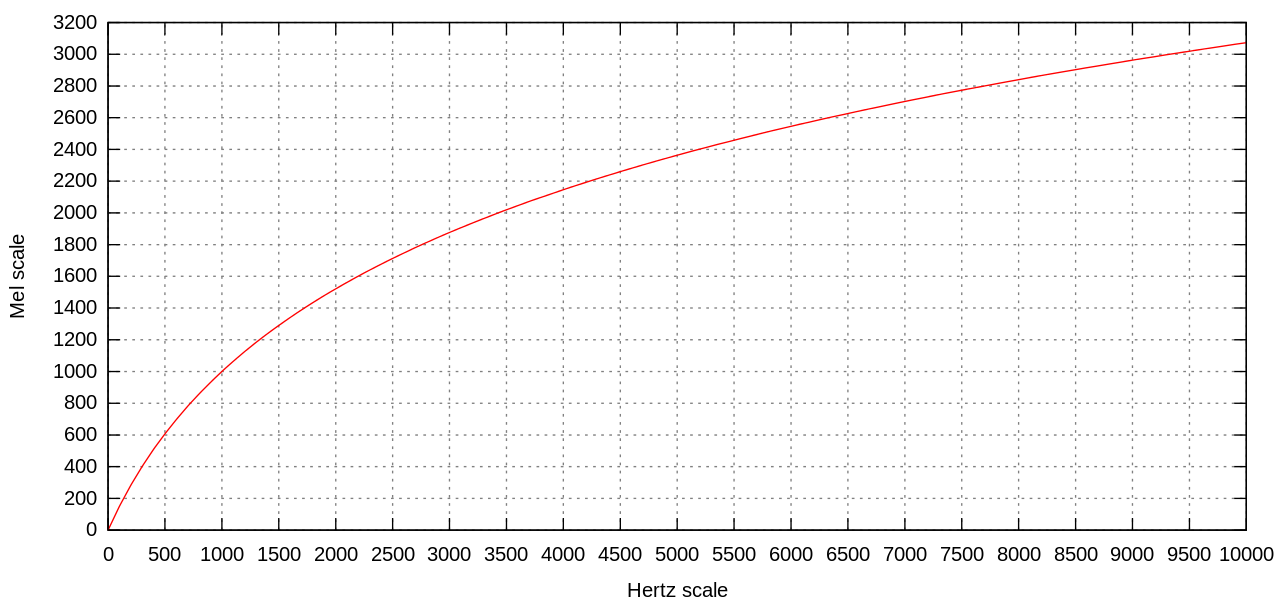
\includegraphics[width=1\textwidth]{Immagini/mel_plot}
	\caption{Grafico della scala mel in funzione della scala in Hertz.}
	\label{fig:mel_plot}
\end{figure}

Per il calcolo dello spettrogramma mel occorre dividere l'input in blocchi usando finestre con overlap, fare la FFT di ogni blocco, generare la scala mel e associare ogni componente spettrale alla relativa frequenza nella scala mel.    

La funzione \texttt{compute\_melspectrogram}, mostrata nel codice~\ref{mel_spectrogram}, usando la libreria \emph{librosa}, calcola gli spettrogrammi da dare in input ai modelli della rete neurale. I file audio, originalmente campionati ad una frequenza di \SI{44.1}{\kilo \hertz}, sono sottocampionati a \SI{16}{\kilo \hertz}. Per calcolare lo spettrogramma, usiamo una lunghezza della finestra di \SI{25}{\milli \second}, un hop size di \SI{10}{\milli \second} e una FFT di \SI{64}{\milli \second}. Lo spettrogramma è contenuto in una matrice di dimensioni $128 \times 51$, poiché il numero di bande mel è 128 e la parola di mezzo secondo viene divisa in finestre da \SI{10}{\milli \second}.

\begin{lstlisting}[language=iPython,firstnumber=1, caption=mel\_spectrogram.py, label=mel_spectrogram,captionpos=b]
import librosa

def compute_melspectrogram(filename, word_center):
    # audio recordings are downsampled to a sampling rate of 16 kHz.
    sample_rate = 16000
    #librosa.load loads the audio file as a floating point time series.
    # y: audio time series, sr: sample rate
    y, _ = librosa.load(path = filename, sr = sample_rate, offset = word_center - 0.25, duration = 0.5)

    # We use a window length of 25 ms, hop size of 10 ms and a fast Fourier
    # transform size of 64 ms.
    window_length = int(0.025*sample_rate)
    hop_size = int(0.01*sample_rate)
    fft_size = int(0.064*sample_rate)
    # For each word instance, we take a half-second context window centered
    # on the word and compute a 128 bin log-mel-spectrogram
    mels_number = 128
    # librosa.feature.melspectrogram computes a mel-scaled spectrogram.
    mel_spectrogram = librosa.feature.melspectrogram(y, sr = sample_rate, n_fft = fft_size, hop_length = hop_size, win_length = window_length, n_mels = mels_number)
    # librosa.power_to_db converts a power spectrogram to a dB-scale
    # spectrogram.
    log_mel_spectrogram = librosa.power_to_db(mel_spectrogram)
    
    return log_mel_spectrogram
\end{lstlisting}

Il risultato della funzione \texttt{log\_mel\_spectrogram} applicato alla parola ``stones'' pronunciata tra \SI{50.35}{\second} e \SI{50.78}{\second} nell'audio contenuto nella cartella ``I can't get no satisfaction'' è mostrato nella figura~\ref{fig:stones_spec}. Come ingresso della funzione viene dato il percorso del file ``audio.ogg'' contenuto nella cartella ``I can't get no satisfaction'' e come centro della parola ``stones'' il tempo $\SI[parse-numbers=false]{\frac{50.78 + 50.35}{2}}{\second}$.

\begin{figure}[h]
	\centering	
	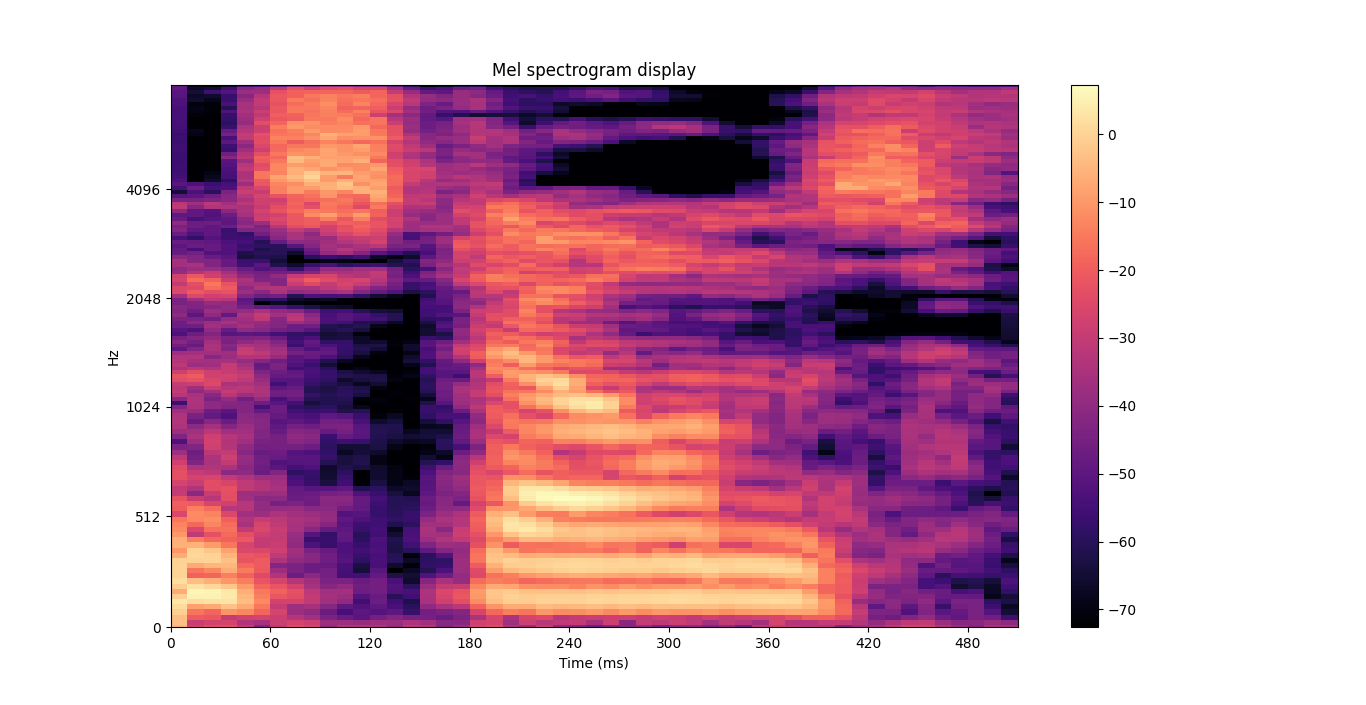
\includegraphics[width=1\textwidth]{../Stones_spectrogram}
	\caption{Spettrogramma di mezzo secondo centrato sulla parola ``stones'' pronunciata nell'audio ``I can't get no satisfaction'' dopo 50.35 secondi.}
	\label{fig:stones_spec}
\end{figure}


\subsection{Creazione delle feature}
\label{subsec:creazione_feature}
Gli spettrogrammi descritti in~\ref{subsec:spettrogramma} sono gli ingressi della rete neurale e sono stati salvati nel preprocessing prima di allenare la rete. Poiché per ogni episodio di training si usa un lettore campionato in modo random dal training set occorre dividere i lettori in training, validation e test. Infine, per ogni lettore occorre salvare gli spettrogrammi delle parole pronunciate. Il codice~\ref{preprocessing} mostra come dividere i lettori e salvare le varie feature. Tra tutti i lettori salvati nel file ``readers\_words.json'' vengono considerati validi solo quelli con almeno due classi, cioè due parole pronunciate e almeno 26 istanze per ogni parola. Questi numeri sono scelti perché in~\cite{Salamon:Few-Shot} vengono proposti diversi modelli a seconda del numero delle classi $C$ e delle istanze $K$ per ogni classe. Il minimo numero di $C$ è pari a 2, mentre il numero minimo di istanze è pari a 26 perché nel training occorre utilizzare 16 istanze per la query e un numero variabile di $K$ che nel caso peggiore è uguale a 10, quindi in totale servirebbero 16+10 istanze della parola. Una volta noti i lettori validi con la funzione \texttt{find\_valid\_readers}, questi vengono ordinati in maniera random prima di dividerli in due gruppi: lettori di training insieme a quelli di validation e lettori di test. La funzione che divide i lettori con un rapporto $138:15:30$ tra training, validation e test si chiama \texttt{create\_training\_validation\_test\_readers}.
I lettori di training e validation saranno poi divisi prima dell'inizio del training.

Le feature, cioè gli spettrogrammi, vengono salvati in due cartelle chiamate ``Training\_validation\_features'' e ``Test\_features'', le quali hanno al loro interno delle cartelle rispettivamente chiamate come il nome del lettore e come il nome dell'articolo di Wikipedia. A sua volta, ogni cartella contiene gli spettrogrammi di ogni istanza della parola.

Il dataset di training e validation viene salvato con la funzione \texttt{save\_dataset}, mentre quello di test con \texttt{save\_test\_dataset}. Il numero massimo di classi e di istanze per ogni classe salvate sono rispettivamente 32 e 64. Questi numeri sono stati scelti perché altrimenti il dataset sarebbe diventato di dimensioni molto grandi.

\begin{lstlisting}[language=iPython,firstnumber=262, caption=preprocessing.py, label=preprocessing,captionpos=b]
min_classes = 2 # minimum number of classes
min_instances_per_class = 26 # minimum number of instances per class

valid_readers = find_valid_readers(min_classes, min_instances_per_class)
# random sample the valid readers
valid_readers = random.sample(valid_readers, len(valid_readers))

# The readers are partitioned into training, validation, and test sets with a 
# 138:15:30 ratio
number_of_training_readers = int(138/183*len(valid_readers))
number_of_test_readers = int(30/183*len(valid_readers))
number_of_validation_readers = int(15/183*len(valid_readers))

# The valid readers are partitioned into training, validation, and test
# readers 
training_validation_readers, test_readers = create_training_validation_test_readers(valid_readers, number_of_training_readers, number_of_test_readers, number_of_validation_readers)
# create the folder for the training and validation features
training_validation_feature_folder_name = "Training_validation_features/"

if not (os.path.exists(training_validation_feature_folder_name)):
    try:
        os.mkdir(training_validation_feature_folder_name)
    except OSError as error:
        print(error)   

max_class_number = 32
max_instances_number = 64

dataset_path = "./Dataset/English spoken wikipedia/english/"
audio_file_name = "audio.ogg"

training_validation_readers = read_json_file("training_validation_readers.json")

save_dataset(training_validation_readers, training_validation_feature_folder_name, dataset_path, audio_file_name, max_class_number, max_instances_number)

reader_paths = read_json_file('readers_paths.json')

# create the folder for the test features
test_feature_folder_name = "Test_features/"

if not (os.path.exists(test_feature_folder_name)):
    try:
        os.mkdir(test_feature_folder_name)
    except OSError as error:
        print(error)   

save_test_dataset(test_readers, reader_paths, test_feature_folder_name, dataset_path, audio_file_name)
\end{lstlisting}

Nella funzione \texttt{find\_valid\_readers} viene letto il file ``readers\_words.json'' e viene creata una lista di dizionari con chiavi ``reader\_name'', ``word'', ``start'', ``end'' e ``folders''. Ogni lettore contiene infatti le parole pronunciate, i relativi timestamp e la cartella in cui è contenuto l'audio che contiene la parola pronunciata. Il dizionario è creato in modo che l'i-esimo valore di ``start'' (o ``end'') corrisponda all'i-esimo valore di ``folders''. I lettori validi sono quelli che pronunciano almeno 2 parole per 26 volte.

\begin{lstlisting}[language=iPython,firstnumber=10, caption=Funzione \texttt{find\_valid\_readers}, label=find_valid_readers,captionpos=b]
def find_valid_readers(min_classes = 2, min_instances_per_class = 26):
    """
    find_valid_readers returns a list of dict with 'word', 'start', 'end'
    and 'folders' keys for each reader name only for the readers with at
    least min_classes words and min_instances_per_class instances per word

    Parameters:
    min_classes (int) (default 2): minimum number of classes per each reader
    min_instances_per_class (int) (default 26): minimum number of instances 
    per class

    Returns:
    valid_readers (list of dict): it contains only the readers with at least
    min_classes words and min_instances_per_class instances per word
    """
    # read the json with the words of each reader
    readers = read_json_file("readers_words.json")

    valid_readers = []

    # for each reader find if it's a valid reader only if he reads C words
    # for K + Q instances
    for reader in readers:    
        valid_words = []
        is_valid_reader = False
        number_of_valid_words = 0

        # for each word of a reader find if there are for K + Q instances
        for word in reader['words']:
            start = []
            end = []
            folders = []

            for item in word['folders']:
                start += item['start']
                end += item['end']
                folders += [item['folder']]*len(item['start'])

            new_word = {'word'   : word['word'], \
                        'start'  : start, \
                        'end'    : end, \
                        'folders': folders}

            # if there are at least 26 (default) instances append a new 
            # valid word
            if (len(new_word['start']) >= min_instances_per_class):
                number_of_valid_words += 1
                valid_words.append(new_word)

        # if the number of valid words is at least min_classes, then the 
        # reader is valid
        if (number_of_valid_words >= min_classes):
            is_valid_reader = True

        # if the reader is valid then add the reader to the valid readers
        # list
        if (is_valid_reader):
            valid_readers.append({'reader_name' : reader['reader_name'],\
                                    'words': valid_words})

    return valid_readers
\end{lstlisting}

La funzione \texttt{create\_training\_validation\_test\_readers} divide i lettori di training e validation da quelli di test usando la variabile \texttt{valid\_readers} creata nel codice~\ref{find_valid_readers}. I primi \texttt{number\_of\_training\_readers} + \texttt{number\_of\_validation\_readers} elementi di \texttt{valid\_readers} sono presi come lettori di training e validation, mentre i restanti come lettori di test.

\begin{lstlisting}[language=iPython,firstnumber=72, caption=Funzione \texttt{create\_training\_validation\_test\_readers}, label=create_training_validation_test_readers,captionpos=b]
def create_training_validation_test_readers(valid_readers, number_of_training_readers, number_of_test_readers, number_of_validation_readers):
    """
    create_training_validation_test_readers split the valid readers into
    training+validation readers and test readers

    Parameters:
    valid_readers (list of dict): list of the valid readers
    number_of_training_readers (int): size of the training readers
    number_of_validation_readers (int): size of the validation readers
    number_of_test_readers (int): size of the test readers

    Returns:
    training_validation_readers (list of dict): it contains the training and
    validation readers splitted from valid_readers
    test_readers (list of dict): it contains the test readers splitted from 
    valid_readers
    """

    # take the first ("number_of_training_readers" + 
    # number_of_validation_readers") elements of "valid_readers" to create
    # the training and validation readers
    training_validation_readers = valid_readers[0 : number_of_training_readers + number_of_validation_readers]

    # take the last "number_of_test_readers" of "valid_readers" to
    # create the test readers
    test_readers = valid_readers[number_of_training_readers + number_of_validation_readers:]

    #write_json_file("training_validation_readers.json", training_readers)
    #write_json_file("test_readers.json", test_readers)

    return training_validation_readers, test_readers
\end{lstlisting}

La funzione \texttt{find\_classes} prende in ingresso un lettore e campiona in modo casuale un numero di parole massimo pari a \texttt{max\_class\_number} e un numero di istanze massimo pari a \texttt{max\_instances\_number}. Ritorna un dizionario con chiavi ``word'', ``start'', ``end'' e ``folders''.

\begin{lstlisting}[language=iPython,firstnumber=100, caption=Funzione \texttt{find\_classes}, label=find_classes,captionpos=b]
def find_classes(reader, max_class_number, max_instances_number):
    """
    find_classes returns classes, a list of dict that has 'word', 'start',
    'end', 'folders' keys.
    'word' value is a string, the word name.
    'start', 'end', 'folders' values are lists. The i-th element of 'start' 
    and 'end' value  corresponds to the i-th element of 'folder' value.
    If the reader contains less words than max_class_number then random 
    sample the words, otherwise random sample max_class_number words.

    Parameters:
    reader (string): one reader from the json file of readers 
    max_class_number (int): maximum class size
    max_instances_number (int): maximum instance size

    Returns:
    classes (list): a list of dict that has 'word', 'start',
    'end', 'folders' keys.
    """
    classes = []

    # taking at most C words from the reader
    # If the reader contains more words than C, random sample C words
    if (len(reader['words']) >= max_class_number):
        reader_words = random.sample(reader['words'], max_class_number)
    # If the reader contains less words than C, random sample the words
    else:
        reader_words = random.sample(reader['words'], len(reader['words']))  

    for word in reader_words:
        # numpy.arange returns evenly spaced values within a given interval.
        # create an array of index to get the start, end and folder of the
        # same index
        index_array = list(numpy.arange(len(word['start'])))
        
        # taking at most max_instances_number instances from each word
        # If the word contains more instances than max_instances_number,
        # random sample max_instances_number instances
        if (len(index_array) >= max_instances_number):
            index_array = random.sample(index_array, max_instances_number)
        # If the word contains less instances than max_instances_number,
        # random sample the index_array
        else:
            index_array = random.sample(index_array, len(index_array))  

        instance_start = []
        instance_end = []
        instance_folder = []
        
        # sample K instances from every C word class
        for index in index_array:
            # get the start, end and folder of the same index
            instance_start.append(word['start'][index])
            instance_end.append(word['end'][index])
            instance_folder.append(word['folders'][index])

        # append the new word of K + Q instances
        classes.append({'word'    : word['word'], \
                        'start'   : instance_start,\
                        'end'     : instance_end, \
                        'folders' : instance_folder})

    return classes
\end{lstlisting}

La funzione \texttt{save\_dataset} salva gli spettrogrammi delle parole di training e validation usando la funzione \texttt{compute\_melspectrogram} presentata nel codice~\ref{mel_spectrogram}. Per ottenere i timestamp delle parole e il relativo audio, necessario alla funzione \texttt{compute\_melspectrogram}, è stato usato \texttt{find\_classes}, presentato nel codice~\ref{find_classes}. 

Gli spettrogrammi sono salvati in un tensore di dimensione $K \times 128 \times 51$, dove $K$ è il numero di volte in cui la parola è stata ripetuta. Il tensore viene salvato il un file con un nome del tipo ``word\_name.pt'', ad esempio ``as.pt'', ``like.pt'', ``the.pt'', ecc.

\begin{lstlisting}[language=iPython,firstnumber=164, caption=Funzione \texttt{save\_dataset}, label=save_dataset,captionpos=b]
def save_dataset(readers, folder_name, dataset_path, audio_file_name, max_class_number, max_instances_number):
    """
    save_dataset saves a pytorch tensor for each word of a reader in a
    folder named as the reader name.

    Parameters:
    readers (list of dict): the list of the training and validation readers saved in training_validation_readers.json
    folder_name (string): name of the folder in which save the features
    dataset_path (string): path of the Spoken Wikipedia Corpora dataset
    audio_file_name (string): name of the ".ogg" audio file 
    max_class_number (int): maximum class size
    max_instances_number (int): maximum instance size

    Returns:
    """
    for reader in tqdm(readers, position = 0):
        if not (os.path.exists(folder_name + reader['reader_name'])):
            try:
                os.mkdir(folder_name + reader['reader_name'])
                classes = find_classes(reader, max_class_number, max_instances_number)
                for item in tqdm(classes, position = 1, leave = False):
                    spectrograms = np.empty([0, 128, 51])
                    for i in range(len(item['start'])):
                        start_in_sec = item['start'][i]/1000 # conversion from milliseconds to seconds
                        end_in_sec = item['end'][i]/1000     # conversion from milliseconds to seconds
                        # calculation of the center time of the word
                        word_center_time = (start_in_sec + end_in_sec)/2
                        # path of the audio file
                        audio_file_path = dataset_path + item['folders'][i] + "/" + audio_file_name
                        if (os.path.exists(audio_file_path)):
                            # compute the 128 bit log mel-spectrogram
                            item_spectrogram = compute_melspectrogram(audio_file_path, word_center_time)
                            # construction of a spectrogram tensor
                            spectrograms = np.concatenate((spectrograms, [item_spectrogram]), axis = 0)
                    # save the spectrograms tensor only if the first dimension is higher than K + Q, 
                    # that is when the word has at least K + Q instances
                    #if (spectrograms.shape[0] >= K + Q):
                        # conversion from numpy array to torch.FloatTensor
                        torch_tensor = torch.FloatTensor(spectrograms)
                        # save the torch tensor
                        torch.save(torch_tensor, folder_name + reader['reader_name'] + "/" + item['word'] + ".pt")
            except OSError as error:
                print(error)   
\end{lstlisting}

La funzione \texttt{save\_test\_dataset} salva gli spettrogrammi delle parole di test. A differenza del codice~\ref{save_dataset} vengono salvate al massimo 16 istanze della parola perché durante il test vengono usate solo $p \in \{1, 5\}$ istanze della parola come \emph{positive set}, mentre tutte le istanze delle altre parole dell'audio compongono il \emph{negative set}.

\begin{lstlisting}[language=iPython,firstnumber=208, caption=Funzione \texttt{save\_test\_dataset}, label=save_test_dataset,captionpos=b]
def save_test_dataset(test_readers, reader_paths, test_feature_folder_name, dataset_path, audio_file_name):
    """
    save_test_dataset saves a pytorch tensor for each word of a test reader in a folder named 
    as the audio of the test reader.

    Parameters:
    test_readers (list of dict): the list of the test readers saved in test_readers.json
    test_feature_folder_name (string): name of the folder in which save the features
    dataset_path (string): path of the Spoken Wikipedia Corpora dataset
    audio_file_name (string): name of the ".ogg" audio file 

    Returns:
    """
    readers_list = []
    audio_folders = []

    for reader in test_readers:
        readers_list.append(reader['reader_name'])

    for reader_name in tqdm(readers_list, position = 0, desc = "test readers"):
        for item in reader_paths:
            if reader_name == item['reader_name']:
                audio_folders += item['folder']

    for audio_folder in tqdm(audio_folders, position = 0, desc = "audio folders"):
        if not (os.path.exists(test_feature_folder_name + audio_folder)):
            try:
                os.mkdir(test_feature_folder_name + audio_folder)
                path = dataset_path + audio_folder + "/target_words.json"
                words = read_json_file(path)
                for word in words:
                    spectrograms = np.empty([0, 128, 51])
                    if (len(word['start']) > 16):
                        indices = random.sample(list(numpy.arange(len(word['start']))), 16)
                    else:
                        indices = random.sample(list(numpy.arange(len(word['start']))), len(word['start']))
                    for i in indices:
                        start_in_sec = word['start'][i]/1000 # conversion from milliseconds to seconds
                        end_in_sec = word['end'][i]/1000     # conversion from milliseconds to seconds
                        # calculation of the center time of the word
                        word_center_time = (start_in_sec + end_in_sec)/2
                        # path of the audio file
                        audio_file_path = dataset_path + audio_folder + audio_file_name
                        if (os.path.exists(audio_file_path)):
                            # compute the 128 bit log mel-spectrogram
                            item_spectrogram = compute_melspectrogram(audio_file_path, word_center_time)
                            # construction of a spectrogram tensor
                            spectrograms = np.concatenate((spectrograms, [item_spectrogram]), axis = 0)
                    # save the spectrograms tensor only if the first dimension is higher than K + Q, 
                    # that is when the word has at least K + Q instances
                    #if (spectrograms.shape[0] >= K + Q):
                        # conversion from numpy array to torch.FloatTensor
                    torch_tensor = torch.FloatTensor(spectrograms)
                    # save the torch tensor
                    torch.save(torch_tensor, test_feature_folder_name + audio_folder + "/" + word['word'] + ".pt")
                
            except OSError as error:
                print(error)   
\end{lstlisting}
\clearpage



\section{Implementazione della Prototypical network}
\label{sec:implementazione_protonet}
\subsection{Definizione della rete}
\label{subsec:definizione_protonet}
La CNN che funge da rete di embedding per la Prototypical Network è costituita da 4 strati convoluzionali, come si può vedere nel codice~\ref{Protonet}. Il primo di essi ha come ingresso un singolo canale e come uscita 64 mentre i tre successivi traspongono 64 canali in altri 64.
Ogni blocco convoluzionale ha 4 fasi:
\begin{itemize}
	\item \texttt{nn.Conv2d(in\_channels,out\_channels,3,padding=1)}: Convoluzione bidimensionale con un kernel 3x3 i cui parametri vengono aggiornati ad ogni backward. Viene effettuato un padding di zeri ai bordi dell'ingresso.
	\item \texttt{nn.BatchNorm2d(out\_channels)}: La batch normalization è un metodo utilizzato per rendere le reti neurali artificiali più veloci e stabili attraverso la normalizzazione degli input dei livelli con re-centering and re-scaling.
	\item \texttt{nn.ReLU()}: il rettificatore è una funzione di attivazione definita come la parte positiva del suo argomento. $f(x)=\max(0,x)$
	\item \texttt{nn.MaxPool2d(2)}: Il max-pooling è un metodo per ridurre la dimensione di un’immagine, suddividendola in blocchi e tenendo solo quello col valore più alto.
\end{itemize}
Al termine dei blocchi viene effettuato il reshape dell'uscita schiacciandola in una sola dimensione, \texttt{x.view(x.size(0),-1)}, in modo da avere una matrice le cui righe rappresentano gli embedding vettoriali.

La funzione \texttt{count\_parameters} ritorna il numero di parametri della rete che, in accordo con~\cite{Salamon:Few-Shot}, devono essere compresi tra $120000$ e $230000$.

\begin{lstlisting}[language=iPython,firstnumber=1, caption=protonet.py, label= Protonet,captionpos=b]
import torch.nn as nn

def count_parameters(model):
    return sum(p.numel() for p in model.parameters() if p.requires_grad)

def conv_block(in_channels,out_channels):

    return nn.Sequential(
        nn.Conv2d(in_channels,out_channels,3,padding=1),
        nn.BatchNorm2d(out_channels),
        nn.ReLU(),
        nn.MaxPool2d(2)
    )

class Protonet(nn.Module):
    def __init__(self):
        super(Protonet,self).__init__()
        self.encoder = nn.Sequential(
            conv_block(1,64),
            conv_block(64,64),
            conv_block(64,64),
            conv_block(64,64)
        )
    def forward(self,x):
        (num_samples,mel_bins, seq_len) = x.shape
        # tensor 3D to tensor 4D with 3rd dimension = 1
        x = x.view(-1,1,mel_bins,seq_len) 
        x = self.encoder(x)
        return x.view(x.size(0),-1)
\end{lstlisting}

\subsection{Training}
Il primo for rappresenta l'inizio degli episodi.
Il numero totale di iterazioni è 60000 come in \cite{Salamon:Few-Shot}; per ogni episodio viene richiamata la funzione \texttt{batch\_sample}.

Con \texttt{loss\_out.backward()} viene utilizzata la loss per la retropropagazione che aggiorna i parametri della rete.

\begin{lstlisting}[language=iPython,firstnumber=1, caption=protonet\_training.py, label=protonet_training main,captionpos=b]
from tqdm import trange, tqdm
import torch
import numpy as np
import scipy
from scipy import io


if torch.cuda.is_available():
  device = torch.device("cuda")
  print("Device: {}".format(device))
  print("Device name: {}".format(torch.cuda.get_device_properties(device).name))
else:
  device = torch.device("cpu")

C = 10 # classes
K = 5 # instances per class
Q = 16 # query set size

model = Protonet()
if torch.cuda.is_available():
  model.to(device='cuda')

print("Model parameters: {}".format(count_parameters(model)))

optim = torch.optim.Adam(model.parameters(), lr = 0.001)

training_readers, validation_readers = get_training_validation_readers("/Training_validation_features/", C)

print ("Training...")

last_accuracy = 0.0
train_loss = []
train_acc = []


# To construct a C-way K-shot training episode, we randomly sample a reader 
# from the training set, sample C word classes from the reader, and sample K
# instances per class as the support set.

for episode in trange(60000, desc = "episode", position = 0, leave = True):
    query, support = batch_sample(training_readers, C, K, Q)
    if torch.cuda.is_available():
      support = support.to(device='cuda')
      query = query.to(device='cuda')
    
    model.train()
    optim.zero_grad()
    loss_out, acc_val = loss(support, query, model)

    loss_out.backward()
    optim.step()
    
    train_loss.append(loss_out.item())
    train_acc.append(acc_val.item())
    
    if (episode+1)%5000 == 0:
      valid_loss = []
      valid_acc = []
      print ("\nValidation...")

      model.eval()

      for validation_episode in range(1000):
          query, support = batch_sample(validation_readers, C, K, Q)
          if torch.cuda.is_available():
            support = support.to(device='cuda')
            query = query.to(device='cuda')
          
          val_loss, acc_val = loss(support, query, model)
          optim.step()
          
          valid_loss.append(val_loss.item())
          valid_acc.append(acc_val.item())

      print("\nValidation accuracy: {}".format(np.mean(valid_acc)))

      if np.mean(valid_acc) > last_accuracy: 

        torch.save({
              'epoch': episode+1,
              'model_state_dict': model.state_dict(),
              'optimizer_state_dict': optim.state_dict(),
              'train_loss': train_loss,
              'train_acc' : train_acc,              
              'valid_loss': valid_loss,
              'valid_acc' : valid_acc,
              'avg_loss_tr' : np.mean(train_loss),
              'avg_acc_tr' : np.mean(train_acc),
              'avg_loss_val' : np.mean(valid_loss),
              'avg_acc_val' : np.mean(valid_acc),
              }, "/Modelli-Prototypical-Network/prototypical_model_C{}_K{}.pt".format(C, K))
        
        last_accuracy = np.mean(valid_acc)

        scipy.io.savemat('/Modelli-Prototypical-Network/prototypical_results_C{}_K{}.mat'.format(C, K), {'train_loss': train_loss , 'train_acc' : train_acc, 'valid_loss':valid_loss,'valid_acc':valid_acc})
\end{lstlisting}

La funzione \texttt{get\_training\_validation\_readers}, a partire dalla lista di lettori di training/validation, seleziona quelli che hanno almeno un numero di parole diverse pari a C e li suddivide tra training e validation seguendo il rapporto usato in \cite{Salamon:Few-Shot}.
Per fare ciò scorre l'elenco delle directory dei lettori e salva su un array le parole a loro associate. Al termine di questa operazione, se il numero di parole è almeno C il lettore è ritenuto valido e il suo nome viene aggiunto a una lista. Infine la lista viene scissa in lettori di training e di validation. 

\begin{lstlisting}[language=iPython,firstnumber=1, caption=get\_training\_validation\_readers, label=get_training_validation_readers,captionpos=b]
def get_training_validation_readers(features_folder, C):
  """
  get_training_validation_readers returns training and validation readers. 
  From the training and validation readers, it takes only the readers with 
  at least C words and split the list in training readers and validation 
  readers.

  Parameters:
  features_folder (list of string): list of the path of the training and validation
  C (int): number of classes

  Returns:
  training_readers (list of string): list of the training readers paths
  validation_readers (list of string): list of the validation readers paths
  """
  readers_path = []
  train_val_readers = []
  # scan each reader folder in the feature_folder
  for entry in os.scandir(features_folder):
      # create a list of reader names
      readers_path.append(entry.path)
  for reader_path in readers_path:
    words = []
    for word in os.scandir(reader_path):
            # create a list containing the path of the words
            words.append(word.path)
    if (len(words) >= C):
      train_val_readers.append(reader_path)
  train_val_readers = random.sample(train_val_readers, len(train_val_readers))
  training_readers = train_val_readers[:int(138/153*len(train_val_readers))]
  validation_readers = train_val_readers[int(138/153*len(train_val_readers)):]
  return training_readers, validation_readers
\end{lstlisting}

La funzione \texttt{batch\_sample} campiona a caso uno dei lettori di training e di questo seleziona casualmente $C$ parole. Per ognuna di queste parole si ricava il numero di istanze presenti del dataset e vengono campionate $K+Q$ istanze random della parola. Le $K+Q$ istanze vengono divise in $K$ istanze del support set e $Q$ stanze del query set. La funzione ritorna due tensori \texttt{query} e \texttt{support}, rispettivamente di dimensioni $C \times Q \times 128 \times 51$ e $C \times K \times 128 \times 51$.

\begin{lstlisting}[language=iPython,firstnumber=1, caption=batch\_sample, label=batch_sample,captionpos=b]
import os
import numpy
import random

def batch_sample(features, C, K, Q = 16):
    """
    batch_sample returns the support and query set. 
    It reads each folder in feature_folder and  load the tensor with the spectrograms of the word.
    Then random sample the instances (spectrograms) of the word to get only K+Q spectrograms. 
    The first K spectrograms compose the support set and the last Q ones compose the query set.

    Parameters:
    features (list): training/validation features paths
    C (int): class size
    K (int): support set size
    Q (int): query set size (default: 16)

    Returns:
    support (torch.FloatTensor): support set
    query (torch.FloatTensor): query set
    """
    # initialize support tensor of dimension 0 x K x 128 x 51
    support = torch.empty([0, K, 128, 51])
    # initialize query tensor of dimension 0 x Q x 128 x 51
    query = torch.empty([0, Q, 128, 51])
    # random sample a reader
    reader = random.sample(features, 1)[0]
    words = []
    # scan the torch tensor saved in each reader folder
    for word in os.scandir(reader):
        # create a list containing the path of the words
        words.append(word.path)
    # random sample C paths of the words of a reader
    words = random.sample(words, C)
    # randomize the instances of each word
    for word in words:
        # load the tensor containing the spectrograms of the instances of
        # one word
        spectrogram_buf = torch.load(word)
        # get the spectrogram tensor shape
        x_dim, y_dim, z_dim = spectrogram_buf.shape
        # get the number of instances
        instances_number = (spectrogram_buf.shape)[0]
        # random sample K + Q indices
        index = random.sample(list(torch.arange(instances_number)), K + Q)
        # initialize the spectrogram tensor
        spectrogram = torch.empty([0, 128, 51])
        for i in index:
            # concatenate spectrogram_buf with spectrogram to get a new
            # tensor of random sampled instances of the word
            spectrogram = torch.cat((spectrogram, (spectrogram_buf[i, :, :]).view(1, y_dim, z_dim)), axis = 0)
        # concatenate the first K spectrograms with the support set
        support =  torch.cat((support, (spectrogram[:K]).view(1, K, y_dim, z_dim)), axis = 0)
        # concatenate the last Q spectrograms with the query set
        query = torch.cat((query, (spectrogram[K:K+Q]).view(1, Q, y_dim, z_dim)), axis = 0)
    return query, support
\end{lstlisting}
Una volta ottenute, le feature del support set e query set vengono date in ingresso alla funzione \texttt{loss}, mostrata nel codice~\ref{protonet_loss}. Entrambi i set vengono ridimensionati, rispettivamente da $C \times K \times 128 \times 51$ a $(C \cdot K) \times 128 \times 51$ e da $C \times Q \times 128 \times 51$ a $(C \cdot Q) \times 128 \times 51$.
Vengono poi concatenate, risultando in un tensore $\left(C \cdot (Q + K)\right) \times 128 \times 51$, per poter essere passate al modello che calcolerà gli embedding per ogni istanza.
Gli elementi del support set che fanno parte della stessa classe andranno a costituire i prototipi tramite una media dei loro valori.

Il parametro \texttt{target\_inds} viene costruito ripetendo l'indice di ogni classe, $0, 1, \dots, C$, per il numero di query, 16, e sarà utilizzato per poter ricavare a che classe appartiene ogni query.

Vengono successivamente calcolate le distanze rispetto ai prototipi degli embedding di ogni classe tramite la funzione \texttt{euclidean\_dist} che ritorna una matrice di dimensioni $(C \cdot Q) \times C$. L'i-esima riga e la j-esima colonna rappresentano la distanza euclidea tra gli embedding della i-esima query ($i = 1, \dots, C \cdot Q$) e quelli del j-esimo ($j = 1, \dots, C$) prototipo.

Per ogni query viene poi usata la funzione di attivazione softmax, definita in~\eqref{eq:softmax}, i cui argomenti sono le distanze tra la query e i prototipi delle varie classi. La funzione loss da minimizzare è il logaritmo del softmax preso con segno negativo, come nell'equazione~\eqref{eq:loss_proto}. Se la query è vicina al prototipo, la funzione softmax tende a 1 e di conseguenza il suo logaritmo a 0, dunque la loss tende a 0, come dovrebbe appunto risultare. Nel caso in cui, invece, la query è molto lontata dal prototipo, la funzione softmax tende a 0 e il suo logaritmo a $-\infty$. In questo caso, la loss, definita come il logaritmo del softmax preso con segno negativo, tende a $+\infty$, come ci si aspetta.

Poiché la funzione \texttt{log\_softmax} di Pytorch ritorna una matrice $(C \cdot Q) \times C$, per ogni riga occorre prendere solo l'elemento relativo alla classe del prototipo. Questo è possibile utilizzando la funzione \texttt{gather} di Pytorch.

L'accuracy invece è determinata dal numero dei casi in cui il prototipo a distanza minima da una query (o il massimo del logaritmo del softmax) corrisponde al prototipo della classe associata alla query.

\begin{lstlisting}[language=iPython,firstnumber=1, caption=protonet\_loss.py, label=protonet_loss,captionpos=b]
import torch
import torch.nn.functional as F

def euclidean_dist(x, y):
    """ 
    euclidean_dist computes the euclidean distance from two arrays x and y

    Parameters:
    x (torch.FloatTensor): query array 
    y (torch.FloatTensor): prototype array

    Returns:
    torch.pow(x - y, 2).sum(2) (double): the euclidean distance from x and y
    """
    # x: N x D
    # y: M x D
    n = x.size(0)
    m = y.size(0)
    d = x.size(1)
    assert d == y.size(1)

    x = x.unsqueeze(1).expand(n, m, d)
    y = y.unsqueeze(0).expand(n, m, d)

    return torch.pow(x - y, 2).sum(2)

def loss(xs, xq, model):
    """
    loss returns the loss and accuracy value. It calculates p_y, the loss 
    softmax over distances to the prototypes in the embedding space. We need
    to minimize the negative log-probability of p_y to proceed the learning
    process.

    Parameters:
    xs (torch.FloatTensor): support set
    xq (torch.FloatTensor): query set
    model (torch.nn.Module): neural network model

    Returns:
    loss_val (double): loss value
    acc_val (double): accuracy value
    """
    # xs = Variable()
    n_class = xs.size(0)
    assert xq.size(0) == n_class
    n_support = xs.size(1)
    n_query = xq.size(1)

    target_inds = torch.arange(0, n_class).view(n_class, 1, 1).expand(n_class, n_query, 1).long()

    if torch.cuda.is_available():
        target_inds = target_inds.to(device='cuda')

    x = torch.cat([xs.view(n_class * n_support, *xs.size()[2:]),
                    xq.view(n_class * n_query, *xq.size()[2:])], 0)
    
    embeddings = model(x)

    embeddings_dim = embeddings.size(-1)
    
    prototypes = embeddings[:n_class*n_support].view(n_class, n_support, embeddings_dim).mean(1)   
    
    queries = embeddings[n_class*n_support:]
    
    dists = euclidean_dist(queries, prototypes)
    
    log_p_y = F.log_softmax(-dists, dim=1).view(n_class, n_query, -1)
    
    loss_val = -log_p_y.gather(2, target_inds).squeeze().view(-1).mean()

    _, y_hat = log_p_y.max(2)
    acc_val = torch.eq(y_hat, target_inds.squeeze()).float().mean()
    
    return loss_val, acc_val
\end{lstlisting}
\subsection{Validation}
\label{subsec:proto_validation}
Ogni 5000 episodi del training vengono effettuati 1000 episodi di validation.
Come nel training vengono ricavati support set e query set, ma in questo caso dai lettori di validation.
Per questi vengono calcolati con la funzione \texttt{loss} allo stesso modo loss e accuracy e vengono salvati.
In questo caso però i parametri del modello non vengono aggiornati.
Questo processo è necessario per verificare l'effettività del modello su ingressi mai visti in fase di training.
Al termine dei 1000 episodi di validation, se la media dell'accuracy è migliore di quella calcolata nel passo precedente il modello viene salvato e sovrascritto, altrimenti viene ignorato. In questo modo si salva il modello migliore durante il training, cercando di evitare sia underfitting sia overfitting.


\subsection{Test}

Nella fase di test, seguendo l'articolo di riferimento, l'oggetto di interesse non sono i lettori come nel caso di training e validation. Un episodio di test è formato da un audio di un lettore di test. Da questi sarà necessario identificare un gruppo di istanze di una parola, il positive set e, campionando nell'audio, si potrà verificare se la rete è in grado di riconoscere la parola designata.


Per ogni audio quindi viene ricavato il numero di parole e le relative istanze.
Per ognuna di esse viene ricavato un positive set e un negative set con i quali è possibile verificare la rete.
Questo processo viene ripetuto 10 volte come in \cite{Salamon:Few-Shot}, in modo da generalizzare il più possibile il test.
Infatti, il positive set è  ricavato campionando casualmente p istanze della parola che si sta analizzando, mentre il negative set è ottenuto campionando n istanze fra tutte le altre parole dello stesso audio.

Le predizioni sono contenute nel vettore \texttt{y\_pred}, mentre in \texttt{y\_true} sono presenti le label reali di ogni query.

La funzione \texttt{precision\_recall\_curve} utilizza \texttt{y\_pred} e \texttt{y\_true} per calcolare precision e recall.
Infine, \texttt{sklearn.metrics.auc} calcola la AUPRC.
Questo calcolo avviene al termine delle operazioni per ogni audio.
Una volta terminati gli audio viene calcolata media e varianza degli AUPRC.

\begin{lstlisting}[language=iPython,firstnumber=77, caption=protonet\_test.py, label=protonet_test,captionpos=b]
def main():
    p = 5
    n = 10

    C = 2
    K = 1

    model = Protonet()
    optim = torch.optim.Adam(model.parameters(), lr = 0.001)

    if torch.cuda.is_available():
        checkpoint = torch.load("Models/Prototypical/prototypical_model_C{}_K{}.pt".format(C, K), map_location=torch.device('cuda'))
    else:
        checkpoint = torch.load("Models/Prototypical/prototypical_model_C{}_K{}.pt".format(C, K), map_location=torch.device('cpu'))
    model.load_state_dict(checkpoint['model_state_dict'])
    optim.load_state_dict(checkpoint['optimizer_state_dict'])


    model.eval()

    if torch.cuda.is_available():
        model.to(device='cuda')

    auc_list = []
    for audio in tqdm(os.scandir("Test_features/"), desc = "Test features"):
        y_pred = []
        y_true = []
        # getting the number of target keywords in each audio
        target_keywords_number = len([name for name in os.listdir(audio) if os.path.isfile(os.path.join(audio, name))])

        for i in range (target_keywords_number):
            for j in range (10):
                negative_set, positive_set, query_set = get_negative_positive_query_set(p, n, i, audio)  

                y_pred_tmp, y_true_tmp = test_predictions(model, negative_set, positive_set, query_set, n, p)
                y_pred_tmp = y_pred_tmp.cpu().tolist()
                y_true_tmp = y_true_tmp.cpu().tolist()
                
                y_pred.extend(y_pred_tmp)
                y_true.extend(y_true_tmp)

        precision, recall, thresholds = sklearn.metrics.precision_recall_curve(y_true, y_pred)
        auc_tmp = sklearn.metrics.auc(recall, precision)
        auc_list.append(auc_tmp)
        
    auc = np.mean(auc_list)
    print("Area under precision recall curve: {}".format(auc))
    auc_std_dev = np.std(auc_list)
    print("Standard deviation area under precision recall curve: {}".format(auc_std_dev))
\end{lstlisting}

Per costruire il positive e negative set viene usata la funzione \texttt{get\_negative\_positive\_query\_set}.
Tramite un indice che indica le istanze della parola appartenente alla classe positiva vengono campionati p spettrogrammi che vanno a costituire il positive set. Le restanti istanze della stessa parola vengono inserite invece nel query set come esempio di spettrogramma che la rete dovrebbe riconoscere.
Tra l'elenco delle parole viene quindi rimossa la parola postiva con \texttt{words.remove(pos\_word)}.
Usando le restanti vengono ricavate n esempi di negative set campionando a caso una delle parole e una delle istanze di essa.
Allo stesso modo viene formata la seconda metà del query set che rappresenta gli esempi negativi. Il numeri di query negative viene preso uguale a quello delle positive.

\begin{lstlisting}[language=iPython,firstnumber=33, caption=Funzione \texttt{get\_negative\_positive\_query\_set}, label=get_negative_positive_query_set,captionpos=b]
def get_negative_positive_query_set(p, n, i, audio):
    # initialize support tensor of dimension p x 128 x 51
    positive_set = torch.empty([0, 128, 51])
    negative_set = torch.empty([0, 128, 51])
    # initialize query tensor of dimension n x 128 x 51
    query_set = torch.empty([0, 128, 51])
    
    words = []
    for word in os.scandir(audio.path):
        words.append(word.path)
        
    pos_word = words[i]

    spectrograms = torch.load(pos_word)
    index = np.arange(spectrograms.shape[0])
    pos_index = random.sample(list(index), p)
    for i in pos_index:
        pos = spectrograms[i, :, :]
        positive_set = torch.cat((positive_set, pos.view(1, 128, 51)), axis = 0)
    for i in index:
        if i not in pos_index:
            query = spectrograms[i, :, :]
            query_set = torch.cat((query_set, query.view(1, 128, 51)), axis = 0)
            
    words.remove(pos_word)

    for i in range(n):
        neg = random.sample(words, 1)
        spectrograms = torch.load(neg[0])
        index = np.arange(spectrograms.shape[0])
        neg_index = random.sample(list(index), 1)
        neg = spectrograms[neg_index, :, :]
        negative_set = torch.cat((negative_set, neg.view(1, 128, 51)), axis = 0)

    for i in range(query_set.shape[0]):
        query_sample = random.sample(words, 1)
        spectrograms = torch.load(query_sample[0])
        index = np.arange(spectrograms.shape[0])
        query_index = random.sample(list(index), 1)
        query = spectrograms[query_index, :, :]
        query_set = torch.cat((query_set, query.view(1, 128, 51)), axis = 0)

    return negative_set, positive_set, query_set
\end{lstlisting}

A questo punto, i tre set e il modello sono passati alla funzione \texttt{test\_predictions}.
Allo stesso modo di training e validation vengono calcolati gli embedding per ogni istanza e i prototipi delle due classi: positive set e negative set.
Vengono calcolate le distanze che sono passate con segno negativo alla funzione \texttt{log\_softmax}. Tra i risultati viene selezionato l'elemento 0 della terza dimesione che rappresenta la probabilità che la query appartenga alla classe positiva.

\begin{lstlisting}[language=iPython,firstnumber=11, caption=Funzione \texttt{test\_prediction}, label=test_predictions,captionpos=b]
def test_predictions(model, negative_set, positive_set, query_set, n, p):
    n_class = 2
    n_query = query_set.size(0)
    
    xs = torch.cat((positive_set, negative_set), 0)   
    x = torch.cat((xs, query_set), 0)
    
    embeddings = model(x)
    embeddings_dim = embeddings.size(-1)
    
    positive_embeddings = embeddings[:p].view(1, p, embeddings_dim).mean(1)    
    negative_embeddings = embeddings[p:p+n].view(1, n, embeddings_dim).mean(1)     
    pos_neg_embeddings =  torch.cat((positive_embeddings, negative_embeddings), 0)
    query_embeddings = embeddings[p+n:]
    dists = euclidean_dist(query_embeddings, pos_neg_embeddings)

    target_inds = torch.arange(n_class-1, -1, step = -1).view(n_class, 1).expand(n_class, int(n_query/2)).long()

    p_y = F.softmax(-dists, dim = 1).view(n_class, int(n_query/2), -1)

    return p_y[:,:,0].view(-1).detach(), target_inds.reshape(1, -1).squeeze()
\end{lstlisting}
\clearpage


\section{Implementazione della Relation network}
\subsection{Definizione della rete}
Le reti neurali necessarie per la relation network sono effettivamente due.

La prima, chiamata \texttt{CNNEncoder} ha lo stesso scopo della rete nella prototypical, ovvero a partire dalle feature in ingresso produce degli embedding che possono essere confrontati.
Anche in questo caso i layer sono 4 e sono costituiti da:
\begin{itemize}
	\item \texttt{nn.Conv2d()}: Convoluzione bidimensionale con un kernel $3 \times 3$ i cui parametri vengono aggiornati ad ogni backward. Viene effettuato un padding di zeri ai bordi dell'ingresso.
	\item \texttt{nn.BatchNorm2d()}: La batch normalization è un metodo utilizzato per rendere le reti neurali artificiali più veloci e stabili attraverso la normalizzazione degli input dei livelli con re-centering and re-scaling.
	\item \texttt{nn.ReLU()}: il rettificatore è una funzione di attivazione definita come la parte positiva del suo argomento. $f(x)=\max(0,x)$
	\item \texttt{nn.MaxPool2d(2)}: Il max-pooling è un metodo per ridurre la dimensione di un’immagine, suddividendola in blocchi e tenendo solo quello col valore più alto.
\end{itemize}
Seguendo le indicazioni in \cite{DBLP:journals/corr/abs-1711-06025} i primi due blocchi hanno padding pari a 0 mentre negli ultimi due padding=1.
Inoltre, per soddisfare le dimensioni necessarie in ingresso alla seconda rete neurale, il Max Pooling è presente solo nei primi 3 layer. Questo concetto sarà approfondito nel capitolo di training.

La seconda rete è detta \texttt{RelationNetwork} e ha lo scopo di confrontare le concatenazioni di embedding per predirre o meno la loro somiglianza.
Essa è costituita da 2 layer di \texttt{nn.Conv2d()}, \texttt{nn.BatchNorm2d()}, \texttt{nn.ReLU()} e \texttt{nn.MaxPool2d(2)} al termine la funzione \texttt{out.view(out.size(0),-1)} ritorna una matrice le cui righe rappresentano gli embedding vettoriali.
In seguito vengono applicati una ulteriore relu e una sigmoide.

\begin{lstlisting}[language=iPython,firstnumber=1, caption=relation\_network.py, label=relation network,captionpos=b]
import torch
import torch.nn as nn
import math
import torch.nn.functional as F

class CNNEncoder(nn.Module):
    """
    CNNEncoder is the embedding module. The architecture consists of 4 
    convolutional block contains a 64-filter 3 X 3 convolution, a batch 
    normalization and a ReLU nonlinearity layer respectively. 
    The first 3 blocks also contain a 2 X 2 max-pooling layer while the last 
    two do not. We do so because we need the output feature maps for further
    convolutional layers in the relation module
    """
    def __init__(self):
        super(CNNEncoder, self).__init__()
        self.layer1 = nn.Sequential(
                        nn.Conv2d(1,64,kernel_size=3,padding=0),
                        nn.BatchNorm2d(64, momentum=1, affine=True),
                        nn.ReLU(),
                        nn.MaxPool2d(2))
        self.layer2 = nn.Sequential(
                        nn.Conv2d(64,64,kernel_size=3,padding=0),
                        nn.BatchNorm2d(64, momentum=1, affine=True),
                        nn.ReLU(),
                        nn.MaxPool2d(2))
        self.layer3 = nn.Sequential(
                        nn.Conv2d(64,64,kernel_size=3,padding=1),
                        nn.BatchNorm2d(64, momentum=1, affine=True),
                        nn.ReLU(),
                        nn.MaxPool2d(2))
        self.layer4 = nn.Sequential(
                        nn.Conv2d(64,64,kernel_size=3,padding=1),
                        nn.BatchNorm2d(64, momentum=1, affine=True),
                        nn.ReLU())
                        #nn.MaxPool2d(2))

    def forward(self,x):
        out = self.layer1(x)
        out = self.layer2(out)
        out = self.layer3(out)
        out = self.layer4(out)
        #out = out.view(out.size(0),-1)
        return out # 64

class RelationNetwork(nn.Module):
    """
    The RelationNetwork is the relation module. It consists of two 
    convolutional blocks and two fully-connected layers. Each of 
    convolutional block is a 3 X 3 convolution with 64 filters followed 
    by batch normalisation, ReLU non-linearity and 2 X 2 max-pooling.
    The two fully-connected layers are 8 and 1 dimensional, respectively. 
    All fully-connected layers are ReLU except the output layer is Sigmoid 
    in order to generate relation scores in a reasonable range for all 
    versions of our network architecture.
    """
    def __init__(self,input_size,hidden_size):
        super(RelationNetwork, self).__init__()
        self.layer1 = nn.Sequential(
                        nn.Conv2d(128,64,kernel_size=3,padding=1),
                        nn.BatchNorm2d(64, momentum=1, affine=True),
                        nn.ReLU(),
                        nn.MaxPool2d(2))
        self.layer2 = nn.Sequential(
                        nn.Conv2d(64,64,kernel_size=3,padding=1),
                        nn.BatchNorm2d(64, momentum=1, affine=True),
                        nn.ReLU(),
                        nn.MaxPool2d(2))
        self.fc1 = nn.Linear(input_size, hidden_size)
        self.fc2 = nn.Linear(hidden_size, 1)

    def forward(self,x):
        out = self.layer1(x)    #  (CLASS_NUM * BATCH_NUM_PER_CLASS * CLASS_NUM) X FEATURE_DIM X 2 X 2
        out = self.layer2(out)  #  (CLASS_NUM * BATCH_NUM_PER_CLASS * CLASS_NUM) X FEATURE_DIM X 1 X 1
        out = out.view(out.size(0),-1)   #  (CLASS_NUM * BATCH_NUM_PER_CLASS * CLASS_NUM) X FEATURE_DIM
        out = F.relu(self.fc1(out))      #  (CLASS_NUM * BATCH_NUM_PER_CLASS * CLASS_NUM) X RELATION_DIM
        #out = F.sigmoid(self.fc2(out)) # deprecated
        out = torch.sigmoid(self.fc2(out))  #  (CLASS_NUM * BATCH_NUM_PER_CLASS * CLASS_NUM) X 1
        return out

def weights_init(m):
    classname = m.__class__.__name__
    if classname.find('Conv') != -1:
        n = m.kernel_size[0] * m.kernel_size[1] * m.out_channels
        m.weight.data.normal_(0, math.sqrt(2. / n))
        if m.bias is not None:
            m.bias.data.zero_()
    elif classname.find('BatchNorm') != -1:
        m.weight.data.fill_(1)
        m.bias.data.zero_()
    elif classname.find('Linear') != -1:
        n = m.weight.size(1)
        m.weight.data.normal_(0, 0.01)
        m.bias.data = torch.ones(m.bias.data.size())
\end{lstlisting}

\subsection{Training}
Come nella rete precedente, il primo passo consiste nel campionare i lettori di training e validation con la funzione \texttt{get\_training\_validation\_readers}.
Le due reti \texttt{CNNEncoder} e \texttt{RelationNetwork} con i rispettivi pesi vengono inizializzate.
Per ogni episodio viene poi campionato un support set e query set per un lettore designato.
Le istanze complessive vengono poi passate alla prima rete per costruire gli embedding.
Gli embedding del support set hanno ora dimensione $(C\cdot K)\times64 \times 15 \times 5$ mentre quelli del query set sono $(C\cdot Q)\times64 \times 15 \times 5$.

Prima di essere passati alla seconda rete questi tensori necessitano di avere le ultime due dimensioni pari a 5.
In questo modo, attraversando due volte lo strato di max pooling passeranno da $5 \times 5$ a $2 \times 2$ e infine a $1 \times 1$.
In seguito al flattening le ultime due dimensioni scompaiono e l'ingresso alla relu ha la dimensione corretta: $(C\cdot Q \cdot C)\times 64$.
Le concatenazioni hanno dimensione $(C\cdot Q \cdot C)\times 64 \times 5 \times 5$, infatti ogni query ($C \times Q$) va concetenata con il vettore che rappresenta ognuna delle classi (C).
Quest'ultimo vettore è ottenuto sommando elemento per elemento gli embedding delle istanze di ogni classe usando \texttt{torch.sum(sample\_features,1).squeeze(1)}.
La rete decisionale restituisce quindi un tensore \texttt{relations} $(C \cdot K \cdot C) \times 1 \times 1$  che viene poi suddiviso in una matrice $(C \cdot Q) \times C$ in cui in ogni riga sono presenti le probabilità che una certa query appartenga ad una determinata classe.
La matrice \texttt{one\_hot\_labels} ha la stessa dimensione di \texttt{relations} ma è costituito da zeri tranne nelle colonne in cui la classe corrisponde realmente alla query, in cui il valore è pari a 1.
Questa rappresenta il risultato ideale che vogliamo in uscita dalla rete.
Usando quindi la funzione \texttt{mse} con parametri \texttt{relations} e \texttt{one\_hot\_labels} otteniamo la loss, calcolata come mean square error, che viene utilizzata per aggiornare i parametri delle due reti con \texttt{loss.backward()}.
\begin{lstlisting}[language=iPython,firstnumber=1, caption=relation\_training.py, label=relation training,captionpos=b]
import torch
import torch.nn as nn
from torch.autograd import Variable
import torch.nn.functional as F
from tqdm import trange, tqdm
import numpy as np
import scipy
from scipy import io

# Hyper Parameters
FEATURE_DIM = 64
RELATION_DIM = 8
CLASS_NUM = 5
SAMPLE_NUM_PER_CLASS = 1
BATCH_NUM_PER_CLASS = 16
EPISODE = 60000
TEST_EPISODE = 1000
LEARNING_RATE = 0.001

if torch.cuda.is_available():
  device = torch.device("cuda")
  print("Device: {}".format(device))
  print("Device name: {}".format(torch.cuda.get_device_properties(device).name))
else:
  device = torch.device("cpu")

training_readers, validation_readers = get_training_validation_readers("/Training_validation_features/", CLASS_NUM)

# init neural network
feature_encoder = CNNEncoder()
relation_network = RelationNetwork(FEATURE_DIM, RELATION_DIM)

feature_encoder.apply(weights_init)
relation_network.apply(weights_init)

if torch.cuda.is_available():
    feature_encoder.to(device='cuda')
    relation_network.to(device='cuda')

feature_encoder_optim = torch.optim.Adam(feature_encoder.parameters(), lr = LEARNING_RATE)
relation_network_optim = torch.optim.Adam(relation_network.parameters(), lr = LEARNING_RATE)

print("Training...")

train_loss = []
validation_loss = []

last_accuracy = 0.0

for episode in tqdm(range(EPISODE), desc = "training episode", position=0):

    # sample datas
    batches, samples = batch_sample(training_readers, CLASS_NUM, SAMPLE_NUM_PER_CLASS, BATCH_NUM_PER_CLASS) # samples: C X K X 128 X 51,  batches: C X Q X 128 X 51
    
    samples = samples.view(CLASS_NUM * SAMPLE_NUM_PER_CLASS, 1, *samples.size()[2:])  # (C X K) X 1 X 51 X 51
    batches = batches.view(CLASS_NUM * BATCH_NUM_PER_CLASS, 1, *batches.size()[2:])   # (C X Q) X 1 X 51 X 51

    if torch.cuda.is_available():
        samples = samples.to(device='cuda')
        batches = batches.to(device='cuda')

    # calculate features
    sample_features = feature_encoder(Variable(samples)) # (CLASS_NUM * SAMPLE_NUM_PER_CLASS) X FEATURE_DIM X 5 X 5

    # resize the images from 15 X 5 to 5 X 5 to get square images
    # interpolate down samples the input to the given size
    sample_features = F.interpolate(sample_features, size = 5)
    sample_features = sample_features.view(CLASS_NUM, SAMPLE_NUM_PER_CLASS, FEATURE_DIM, 5, 5) # CLASS_NUM X SAMPLE_NUM_PER_CLASS X FEATURE_DIM X 5 X 5
    sample_features = torch.sum(sample_features,1).squeeze(1)   # CLASS_NUM X FEATURE_DIM X 5 X 5

    batch_features = feature_encoder(Variable(batches)) # (CLASS_NUM * BATCH_NUM_PER_CLASS) X FEATURE_DIM X 5 X 5
    batch_features = F.interpolate(batch_features, size = 5)

    # calculate relations
    # each batch sample link to every samples to calculate relations
    sample_features_ext = sample_features.unsqueeze(0).repeat(CLASS_NUM * BATCH_NUM_PER_CLASS, 1, 1, 1, 1) # (CLASS_NUM * BATCH_NUM_PER_CLASS) X 5 X FEATURE_DIM X 5 X 5
    batch_features_ext = batch_features.unsqueeze(0).repeat(CLASS_NUM, 1, 1, 1, 1)  # 5 X (CLASS_NUM * BATCH_NUM_PER_CLASS) X FEATURE_DIM X 5 X 5
    batch_features_ext = torch.transpose(batch_features_ext, 0, 1)  #  (CLASS_NUM * BATCH_NUM_PER_CLASS) X 5 X FEATURE_DIM X 5 X 5

    relation_pairs = torch.cat((sample_features_ext,batch_features_ext), 2).view(-1, FEATURE_DIM*2, 5, 5)  #  (CLASS_NUM * BATCH_NUM_PER_CLASS * 5) X (FEATURE_DIM * 2) X 5 X 5
    relations = relation_network(relation_pairs).view(-1,CLASS_NUM) #  (CLASS_NUM * BATCH_NUM_PER_CLASS) X CLASS_NUM

    mse = nn.MSELoss()
    
    one_hot_labels = Variable(torch.zeros(BATCH_NUM_PER_CLASS*CLASS_NUM, CLASS_NUM))

    for i in range(CLASS_NUM):
        for j in range(BATCH_NUM_PER_CLASS):
            one_hot_labels[BATCH_NUM_PER_CLASS*i+j,i] = 1

    if torch.cuda.is_available():
        mse = mse.to(device='cuda')
        one_hot_labels = one_hot_labels.to(device='cuda')

    loss = mse(relations,one_hot_labels)

    # training

    feature_encoder.zero_grad()
    relation_network.zero_grad()

    loss.backward()

    torch.nn.utils.clip_grad_norm_(feature_encoder.parameters(), 0.5)
    torch.nn.utils.clip_grad_norm_(relation_network.parameters(), 0.5)

    feature_encoder_optim.step()
    relation_network_optim.step()

    train_loss.append(loss.item())

    if (episode+1)%5000 == 0:
      total_rewards = 0
      #for i in tqdm(range(TEST_EPISODE), desc = "validation episode", position = 1, leave = False):
      for validation_episode in range(TEST_EPISODE):
        # sample datas
        batches, samples = batch_sample(validation_readers, CLASS_NUM, SAMPLE_NUM_PER_CLASS, BATCH_NUM_PER_CLASS) # samples: C X K X 128 X 51,  batches: C X Q X 128 X 51
        
        samples = samples.view(CLASS_NUM * SAMPLE_NUM_PER_CLASS, 1, *samples.size()[2:])  # (C X K) X 1 X 51 X 51
        batches = batches.view(CLASS_NUM * BATCH_NUM_PER_CLASS, 1, *batches.size()[2:])   # (C X Q) X 1 X 51 X 51

        if torch.cuda.is_available():
            samples = samples.to(device)
            batches = batches.to(device)

        # calculate features
        sample_features = feature_encoder(Variable(samples)) # (CLASS_NUM * SAMPLE_NUM_PER_CLASS) X FEATURE_DIM X 5 X 5

        # resize the images from 15 X 5 to 5 X 5 to get square images
        # interpolate down samples the input to the given size
        sample_features = F.interpolate(sample_features, size = 5)
        sample_features = sample_features.view(CLASS_NUM, SAMPLE_NUM_PER_CLASS, FEATURE_DIM, 5, 5) # CLASS_NUM X SAMPLE_NUM_PER_CLASS X FEATURE_DIM X 5 X 5
        sample_features = torch.sum(sample_features,1).squeeze(1)   # CLASS_NUM X FEATURE_DIM X 5 X 5

        batch_features = feature_encoder(Variable(batches)) # (CLASS_NUM * BATCH_NUM_PER_CLASS) X FEATURE_DIM X 5 X 5
        batch_features = F.interpolate(batch_features, size = 5)

        # calculate relations
        # each batch sample link to every samples to calculate relations
        sample_features_ext = sample_features.unsqueeze(0).repeat(CLASS_NUM * BATCH_NUM_PER_CLASS, 1, 1, 1, 1) # (CLASS_NUM * BATCH_NUM_PER_CLASS) X 5 X FEATURE_DIM X 5 X 5
        batch_features_ext = batch_features.unsqueeze(0).repeat(CLASS_NUM, 1, 1, 1, 1)  # 5 X (CLASS_NUM * BATCH_NUM_PER_CLASS) X FEATURE_DIM X 5 X 5
        batch_features_ext = torch.transpose(batch_features_ext, 0, 1)  #  (CLASS_NUM * BATCH_NUM_PER_CLASS) X 5 X FEATURE_DIM X 5 X 5

        relation_pairs = torch.cat((sample_features_ext,batch_features_ext), 2).view(-1, FEATURE_DIM*2, 5, 5)  #  (CLASS_NUM * BATCH_NUM_PER_CLASS * 5) X (FEATURE_DIM * 2) X 5 X 5
        relations = relation_network(relation_pairs).view(-1,CLASS_NUM) #  (CLASS_NUM * BATCH_NUM_PER_CLASS) X CLASS_NUM

        _,predict_labels = torch.max(relations.data,1)

        test_labels = torch.arange(CLASS_NUM).expand(BATCH_NUM_PER_CLASS,CLASS_NUM).transpose(1,0).reshape(-1)

        rewards = [1 if predict_labels[j]==test_labels[j] else 0 for j in range(CLASS_NUM*BATCH_NUM_PER_CLASS)]

        total_rewards += np.sum(rewards)

      valid_accuracy = total_rewards/1.0/CLASS_NUM/BATCH_NUM_PER_CLASS/TEST_EPISODE

      print("\nTest accuracy: {}".format(valid_accuracy))

      if valid_accuracy > last_accuracy:
        torch.save({
                    'epoch': episode+1,
                    'feature_encoder_state_dict': feature_encoder.state_dict(),
                    'relation_network_state_dict' : relation_network.state_dict(),
                    'feature_encoder_optim_state_dict': feature_encoder_optim.state_dict(),
                    'relation_network_optim_state_dict': relation_network_optim.state_dict(),
                    'train_loss': train_loss,
                    'avg_loss_tr' : np.mean(train_loss),
                    'valid_acc' : valid_accuracy,
                    'avg_acc_val' : np.mean(valid_accuracy),
                    }, "/Modelli-Relation-Network/relation_model_C{}_K{}.pt".format(CLASS_NUM, SAMPLE_NUM_PER_CLASS))
        last_accuracy = valid_accuracy

        scipy.io.savemat('/Modelli-Relation-Network/relation_results_C{}_K{}.mat'.format(CLASS_NUM, SAMPLE_NUM_PER_CLASS), {'train_loss': train_loss ,'valid_accuracy':valid_accuracy})

print('Average train loss: {}'.format(np.mean(train_loss)))
\end{lstlisting}


\subsection{Validation}
Come nel capitolo~\ref{subsec:proto_validation}, ogni 5000 episodi di training ne vengono effettuati 1000 di validation. Allo stesso modo del validation della prototypical network, vengono utilizzati lettori di validation sconosciuti alla rete e, nel caso in cui la validation produca una accuracy migliore di quella precedente, il modello viene salvato.
Per fare ciò viene utilizzato un array \texttt{reward} che contiene 1 se la label della j-esima predizione è uguale alla label della j-esima query, altrimenti 0. Successivamente, vengono sommati gli elementi di questo vettori e salvati nella variabile \texttt{total\_rewards}. Per ogni episodio di validation, all'aumentare del numero di predizioni corrette, la variabile \texttt{total\_rewards} tende a $C \cdot Q$.

L'accuracy equivale al numero di volte in cui la predizione è corretta, cioè \texttt{total\_rewards}, diviso il totale delle $C \cdot Q$ query, mediato nei 1000 episodi di validation, come mostrato nella formula~\eqref{eq:acc_relation}.
\begin{equation}\label{eq:acc_relation}
\text{accuracy} = \dfrac{\text{total rewards}}{C \cdot Q \cdot 1000}
\end{equation}
\subsection{Test}
Anche in questo il test ha come oggetto di analisi i singoli audio del dataset e non i lettori. Le fasi del test sono analoghe alla Prototypical network, ma cambia la funzione che calcola le predizioni \texttt{test\_predictions}.
Come in precedenza, il positive set, il negative set e il query set sono passati in ingresso alla prima rete che ne calcola gli embedding.

\begin{lstlisting}[language=iPython,firstnumber=99, caption=relation\_test.py, label=relation test,captionpos=b]
def main():
    p = 5
    n = 10

    C = 2
    K = 5

    FEATURE_DIM = 64
    RELATION_DIM = 8

    feature_encoder = CNNEncoder()
    relation_network = RelationNetwork(FEATURE_DIM, RELATION_DIM)

    if torch.cuda.is_available():
        checkpoint = torch.load("Models/Relation/relation_model_C{}_K{}.pt".format(C, K), map_location=torch.device('cuda'))
    else:
        checkpoint = torch.load("Models/Relation/relation_model_C{}_K{}.pt".format(C, K), map_location=torch.device('cpu'))
    feature_encoder.load_state_dict(checkpoint['feature_encoder_state_dict'])
    relation_network.load_state_dict(checkpoint['relation_network_state_dict'])


    feature_encoder.eval()
    relation_network.eval()

    if torch.cuda.is_available():
        feature_encoder.to(device='cuda')
        relation_network.to(device='cuda')

    auc_list = []
    for audio in tqdm(os.scandir("Test_features/"), desc = "Test features"):
        y_pred = []
        y_true = []
        # getting the number of target keywords in each audio
        target_keywords_number = len([name for name in os.listdir(audio) if os.path.isfile(os.path.join(audio, name))])

        for i in range (target_keywords_number):
            for j in range (1):
                negative_set, positive_set, query_set = get_negative_positive_query_set(p, n, i, audio)

                negative_set = negative_set.view(1 * n, 1, *negative_set.size()[1:])  
                positive_set = positive_set.view(1 * p, 1, *positive_set.size()[1:]) 
                query_set = query_set.view(int(C * query_set.size()[0]/2), 1, *query_set.size()[1:])   # (C X Q) X 1 X 51 X 51
                
                y_pred_tmp, y_true_tmp = test_predictions(feature_encoder,relation_network, positive_set, negative_set, query_set, n, p)

                y_pred.extend(y_pred_tmp)
                y_true.extend(y_true_tmp)

        precision, recall, thresholds = sklearn.metrics.precision_recall_curve(y_true, y_pred)
        auc_tmp = sklearn.metrics.auc(recall, precision)
        auc_list.append(auc_tmp)
        
    auc = np.mean(auc_list)
    print("Area under precision recall curve: {}".format(auc))
    auc_std_dev = np.std(auc_list)
    print("Standard deviation area under precision recall curve: {}".format(auc_std_dev))
\end{lstlisting}

Nella funzione \texttt{test\_predictions} la dimensione del tensore in uscita dalla prima rete passa da $(C \cdot Q) \times 64 \times 15 \times 5$ a $(C \cdot Q) \times 64 \times 5 \times 5$. Successivamente, il positive e negative set vengono concatenati in quanto svolgono il ruolo delle classi con cui confrontare la query.
Tutte le query vengono quindi concatenate con i vettori rappresentanti delle due classi producendo un numero di concatenazioni pari al numero di query moltiplicato per 2 (ovvero il doppio delle istanze rimanenti nella classe positiva dopo la creazione del positive set).

Questo tensore viene poi passato alla rete che calcola le predizioni su quale delle classi (positive set e negative set) sia più simile alla query. In questo modo la rete produce una coppia di valori che indicano la probabilità con cui una query è associata ai due set.
Di questi viene presa solo l'elemento 0 che indica l'affinità con il positive set.
Utilizzando poi un corrispettivo valore che contiene il valore atteso reale è possibile calcolare precision, recall e AUPRC.
\begin{lstlisting}[language=iPython,firstnumber=1, caption=Funzione \texttt{test\_predictions}, label=test_predictions_relation,captionpos=b]
def test_predictions(feature_encoder,relation_network, positive_set, negative_set, query_set, n, p):
    n_class = 2
    n_query = query_set.size(0)

    FEATURE_DIM = 64

    pos_embeddings = feature_encoder(Variable(positive_set)) # (CLASS_NUM * SAMPLE_NUM_PER_CLASS) X FEATURE_DIM X 15 X 5

    # resize the images from 15 X 5 to 5 X 5 to get square images
    # interpolate down samples the input to the given size
    pos_embeddings = F.interpolate(pos_embeddings, size = 5)
    pos_embeddings = pos_embeddings.view(1, p, FEATURE_DIM, 5, 5) # CLASS_NUM X SAMPLE_NUM_PER_CLASS X FEATURE_DIM X 5 X 5
    pos_embeddings = torch.sum(pos_embeddings,1).squeeze(1)   # CLASS_NUM X FEATURE_DIM X 5 X 5

    neg_embeddings = feature_encoder(Variable(negative_set)) # (CLASS_NUM * SAMPLE_NUM_PER_CLASS) X FEATURE_DIM X 5 X 5

    # resize the images from 15 X 5 to 5 X 5 to get square images
    # interpolate down samples the input to the given size
    neg_embeddings = F.interpolate(neg_embeddings, size = 5)
    neg_embeddings = neg_embeddings.view(1, n, FEATURE_DIM, 5, 5) # CLASS_NUM X SAMPLE_NUM_PER_CLASS X FEATURE_DIM X 5 X 5
    neg_embeddings = torch.sum(neg_embeddings,1).squeeze(1)   # CLASS_NUM X FEATURE_DIM X 5 X 5
    
    batch_features = feature_encoder(Variable(query_set)) # (CLASS_NUM * BATCH_NUM_PER_CLASS) X FEATURE_DIM X 5 X 5
    batch_features = F.interpolate(batch_features, size = 5)
    
    pos_neg_embeddings =  torch.cat((pos_embeddings, neg_embeddings), 0)

    # calculate relations
    # each batch sample link to every samples to calculate relations
    pos_neg_embeddings_ext = pos_neg_embeddings.unsqueeze(0).repeat(int(n_class * n_query/2), 1, 1, 1, 1) # (CLASS_NUM * BATCH_NUM_PER_CLASS) X 5 X FEATURE_DIM X 5 X 5
    
    batch_features_ext = batch_features.unsqueeze(0).repeat(n_class, 1, 1, 1, 1)  # 5 X (CLASS_NUM * BATCH_NUM_PER_CLASS) X FEATURE_DIM X 5 X 5
    batch_features_ext = torch.transpose(batch_features_ext, 0, 1)  #  (CLASS_NUM * BATCH_NUM_PER_CLASS) X CLASS_NUM X FEATURE_DIM X 5 X 5

    relation_pairs = torch.cat((pos_neg_embeddings_ext,batch_features_ext), 2).view(-1, FEATURE_DIM*2, 5, 5)  #  (CLASS_NUM * BATCH_NUM_PER_CLASS * CLASS_NUM) X (FEATURE_DIM * 2) X 5 X 5
    relations = relation_network(relation_pairs).view(-1,n_class) #  (CLASS_NUM * BATCH_NUM_PER_CLASS) X CLASS_NUM
    
    target_inds = torch.arange(n_class-1, -1, step = -1).view(n_class, 1).expand(n_class, int(n_query/2)).long()
    
    return relations[:,0].view(-1).detach(), target_inds.reshape(1, -1).squeeze()
\end{lstlisting}

\clearpage

\section{Risultati}
\subsection{Area under precision-recall curve (AUPRC)}
Nella fase di test, la rete elabora una predizione dell'output a partire da un ingresso noto che poi viene confrontata con il valore effettivo.
Nel nostro caso è presente un positive set e un negative set, si tratta quindi di classificazione binaria.
Il confronto tra predizione e label può produrre quattro risultati:
\begin{itemize}
	\item Vero Negativo (TN): il valore reale è negativo e il valore predetto è negativo;
	\item Vero Positivo (TP): il valore reale è positivo e il valore predetto	è positivo;
	\item Falso Negativo (FN): il valore reale è positivo e il valore predetto è negativo;
	\item Falso Positivo (FP): il valore reale è negativo e il valore predetto	è positivo;
\end{itemize}
Questi valori vanno a comporre la confusion matrix.
Nel nostro caso siamo interessati a Precision e Recall.

Il parametro Precision rappresenta quanti tra i casi predetti come positivi sono realmente positivi.

Il parametro Recall indica quanti tra i casi realmente positivi è stato predetto in modo corretto.
\begin{equation}
Precision=\frac{TP}{TP+FP}
\end{equation}
\begin{equation}
Recall=\frac{TP}{TP+FN}
\end{equation}

Consideriamo un vettore contenente le probabilità che una serie di query appartengano a una classe. Impostando una soglia di decisione e confrontando con un altro vettore contenente i valori desiderati, 1 se la query corrisponde alla classe positiva e 0 altrimenti, è possibile ottenere una coppia di valori di precision e recall.

A questo punto ordiniamo il vettore con valori decrescenti.
Consideriamo come soglia il valore di probabilità presente al primo elemento e calcoliamo precision e recall.
Poi, spostiamo la soglia al valore del secondo elemento e calcoliamo altri valori.
Continuando in questo modo si può ottenere una curva considerando alle ascisse i valori di recall e come ordinate i valori di precision.

Calcolando l'area sottesa dalla curva si ricava il valore detto Area under precision-recall curve (AUPRC).
Questo valore è molto utile quando i dati sono sbilanciati e, in una classificazione binaria, siamo più interessati al riconoscimento di una classe in particolare.
\clearpage

\section{Conclusioni}
\clearpage

\nocite{*}
%Il comando \printbibliography produce la sezione bibliografica con relativi
%titolo e testatina. Per mandarne il relativo titolo nell’indice generale si
%usa l’istruzione:
\printbibliography
\end{document} 